\chapter[Объект и метод]{Объект и методы исследования}
\label{cha:objectandmethod}

\section{Цифровые экосистемы}
Появление цифровых экосистем является результатом естественного развития научного сотрудничества и информационных технологий. 
Целью цифровых экосистем является повышение эффективности связей между внутренними и внешними агентами для поддержания бизнеса. 
В литературе есть два широких определения концепции цифровых экосистем. 
Первое исходит из структурной и функциональной перспективы, которая видит цифровую экосистему как открытую сетевую среду для эффективного взаимодействия. Второе, напротив, рассматривает цифровую экосистему как открытый кластер слабо связанных компонент, в котором каждый агент является проактивным для собственной выгоды (Рис. \ref{fig:om0}).

\begin{figure}[H]
  \label{fig:om0}
  \centering
  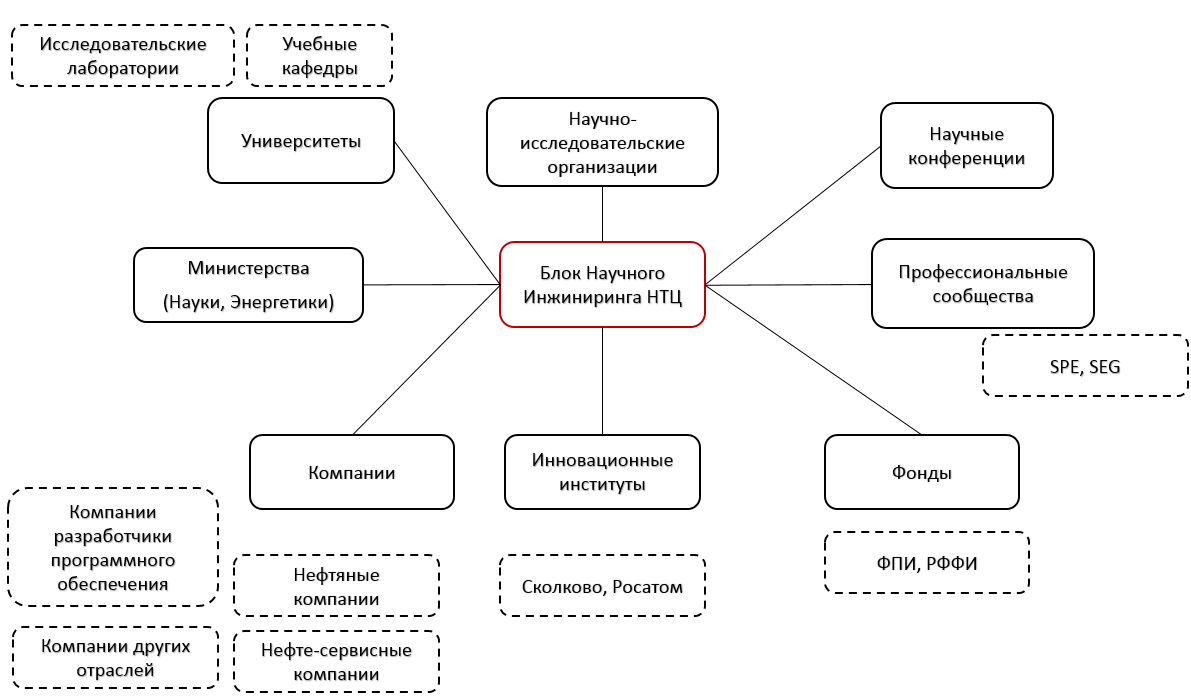
\includegraphics[width=0.8\textwidth]{se_eco}
  \caption{Экосистема научного инжиниринга}
\end{figure}

Понятие ``цифровые артефакты'' вошло в обиход вместе с понятием цифровой экосистемы. 
В широком смысле цифровые артефакты являются синонимами любых информационных результатов действий цифровой экосистемы. 
По своей информационной природе цифровые артефакты могут сохраняться или разрушаться.
Как при сохранении, так и при разрушении происходит видоизменение изначального цифрового артефакта. 
В исторической перспективе цифровые артефакты могут быть изучены, как и любые другие продукты деятельности человека.

Цифровые экосистемы можно рассматривать на макроуровне (страна, отрасль) и на микроуровне (корпорация, группа компаний, отдельное предприятие, департамент). Цифровые артефакты также могут существовать на разных уровнях. 

Одним из примеров цифровых артефактов на микроуровне являются системы распространения знаний в нефтегазовых компаниях.
Система распространения знаний (СРЗ) – это инструмент, помогающий координировать процессы управления и обмена знаниями в области разведки и добычи нефти внутри группы компаний ``Газпром нефть'' для решения технологических и производственных задач при принятии решений. 

Она предназначена для настройки процессов сбора, обработки и распространения знаний с целью извлечения максимальной выгоды от внедряемых в компании практик и технологий.
СРЗ реализована в виде информационной системы с несколькими модулями, помогающими получить необходимую информацию по разным аспектам работы на месторождении. 

В СРЗ систематизировано представлена информация о лучших практиках, применяемых в ``Газпром нефти'' в области разведки и добычи. Система позволяет пользователю проводить сравнительный анализ и подбор оптимальных технических решений в соответствии с необходимыми ему критериями. В ней также хранятся данные обо всех проведенных внутри компании испытаниях нового оборудования, что позволяет наиболее эффективно внедрять новое оборудование и технологии на любом месторождении внутри компании. 

Наибольший вклад в развитие СРЗ вносят эксперты Научно-Технического Центра ``Газпром нефти''. Они формируют крупную структурированную базу знаний по различным областям геологии, геологоразведки и добычи, к которой имеют доступ все сотрудники ``Газпром нефти''. СРЗ – это один из инструментов создания инновационного климата внутри компании, необходимого для развития новых, более эффективных технологий разведки и добычи нефти. 

\section{Модели и моделирование социотехнических объектов}

Современная парадигма научного исследования заключается в том, что реальные объекты заменяются на их упрощённые представления, абстракции, выбираемые так, чтобы в них отражалась сущность явления, те свойства исходных объектов, которые являются существенными для решения проблемы, которая была поставлена. 
Объект, который построен вследствие упрощения, называют моделью.

Модели могут классифицироваться по разным признакам: динамические и статические, дискретные и непрерывные, стохастические и детерминированные, имитационные и аналитические. 

Статистические модели оперируют характеристиками и объектами, которые не меняются во времени. 
В динамических моделях изменение параметров модели во времени является существенным.
Статистические модели имеют дело с уравнениями балансового типа, установившимися процессами, с предельными характеристиками.
Моделирование динамических систем заключается в имитации правил перехода системы из определённого состояния в другое в течение времени.

Модели, у которых состояние изменяется непрерывно во времени, называются непрерывными. 
Модели, у которых переходы от одного состояния системы в другое происходят мгновенно, в дискретные моменты времени, называются дискретными.

Стохастические модели, в отличие от детерминированных, учитывают вероятностный характер параметров системы.

При аналитическом моделировании процессы функционирования исследуемой системы отражаются как алгебраические, интегральные, дифференциальные уравнения и логические соотношения, и в определённых случаях анализ таких соотношений может выполняться посредством аналитических преобразований.

При имитационном моделировании структура моделируемой системы -- её связи и подсистемы -- непосредственным образом представлена структурой модели, а процесс функционирования подсистем в виде уравнений и правил, которые связывают переменные, имитируются на компьютере.

Компьютерные системы предсказательного моделирования (которые также называются системами поддержки принятия инженерных решений) с компьютерными системами проектирования давно применяются в целях автоматизации трудовой деятельности инженера-проектировщика и повышения качества решений, которые принимаются. 
Но до начала XXI века в предсказательном моделировании применялись исключительно математические модели, основанные на принципах физики, описывающие физические явления и процессы, которые происходят при функционировании объекта, сложными дифференциальными уравнениями в частных производных с граничными условиями. 
В содержательных ситуациях для таких уравнений неизвестны ни теоремы о единственности и существовании решения, ни характер зависимости решения от граничных условий и параметров.
Численные методы решения этих уравнений обладают значительной вычислительной трудоёмкостью и самих расчётов, и подготовки исходных данных и расчётных сеток.
В силу этого существенно сокращаются возможности использования этих моделей в проектировании сложных объектов, в особенности на этапе концептуального или предварительного проектирования, когда рассматривается значительное число разных вариантов решений и особенно высока цена решения, которое выбрано неправильно. 
Важная часть предсказательного моделирования -- это имитационное моделирование, которое используется для исследования сложных информационно-телекоммуникационных систем.

\subsection{Апостериорный и априорный подходы к исследованию}
Рассматривая возможности апостериорного и априорного подхода к исследованию, автор склоняется к тому, чтобы отдать первенство экспериментальному изучению данного явления, а потом выяснить, какие из теорий смогут составить базу для дальнейшего углубления в изучение феномена соавторства.

Современные возможности прямого имитационного моделирования стали настолько удобны для произведения вычислительных экспериментов, что для начального подхода к изучению сложных социальных явлений достаточно быстро могут дать исследователю существенное понимание их природы. Формализм математической модели в данном случае не абстрагирует в мир греческих букв, а приближает к пониманию родовых особенностей исследуемого объекта.

Модель стремиться дать то описание системы, для которого она создается. 
Но отметим, что создание модели для полного описания социальной системы не является корректной постановкой задачи. 
Полная модель социальной системы будет настолько же сложна, насколько и сама социальная система. 
Сформулируем следующее определение модели социальной системы (О\ref{defi:so1}):

\begin{defi}[О\ref{defi:so1}] \label{defi:so1}
Модель  $\mathbb{M}_{\Omega}$ социальной системы $\Omega$ может быть использована для получения характеристик $\mathbb{RE}$ с некоторой точностью $\delta$.
\end{defi}

Таким образом, целью модели является получение ответов на некоторую совокупность вопросов. 
Эти вопросы неявно присутствуют (подразумеваются) в процессе анализа, и, следовательно, они руководят созданием модели и направляют его. 
Это означает, что сама модель должна будет дать ответы на эти вопросы с заданной степенью точности. 
Если модель отвечает не на все вопросы или ее ответы недостаточно точны, то говорят, что модель не достигла своей цели.

Агентное моделирование предполагает имитацию поведения системы путем настройки поведения отдельных агентов. 
На основании результатов поведения отдельных индивидов складывается комплексная картина взаимодействий. 
Метод агентного моделирования используется в дополнение к методу системной динамики, в рамках которой моделируется поведение всей системы в целом.

Программные алгоритмы агентного моделирования разработаны в нескольких информационных системах, в частности Anylogic и NetLogo.
Для решения практических задач эти информационные системы используется в социальных науках, в том числе в экономике и социологии. 
Важной задачей агентного моделирования является включение информации о взаимодействиях агентов между собой, так как в некоторых социальных системах именно комплексная структура взаимодействий индивидуальных агентов и приводит к более сложным макро-состояниям. 
Агентное моделирование используется для изучения динамики социальных сетей и взаимного влияния экзогенных и структурных характеристик друг на друга.

Модель для исследования взаимодействия агентов в процессе создания научных статей была реализована автором в программной среде агентного моделирования AnyLogic, базирующемся на языке Java. 
В среде AnyLogic для каждого из агентов прописываются определенные правила поведения – эвристики, индивидуальные стратегии.
После того, как для каждого из агентов прописываются все правила поведения, запускается серия симуляций.
Программные среды для агентного моделирования используются для предсказания коллективного поведения, массовых мероприятий, учебного процесса и многих других социальных процессов.

Для моделирования процессов в данном исследовании использовался метод имитационного моделирования на основе внутренних состояний и действий.
Основное преимущество данного подхода состоит в возможности проведения компьютерного эксперимента для понимания поведения системы в целом с помощью настройки графов состояний и действий децентрализованных индивидуальных агентов. 
Таким образом, в результате была получена база данных поведения агентов для исследования процессов.

В рамках изложенной выше методологии были сформулированы следующие вопросы для исследований:
\begin{enumerate}
\item В какой степени научная статья отражает проведенную НИР? Можно ли судить о качестве НИР по опубликованным научным исследованиям?
\item Каковы социальные механизмы объединения исследователей для проведения НИР? Какие виды компетенций и в какой степени влияют на такое объединение?
\item Как зависит время проведения НИР от количества участвующих исследователей? Существуют ли естественные ограничения на количество и состав исследовательских групп и на чем они основаны?
\item Каковы эвристические алгоритмы поведения исследователей по отношению к издательствам и программным комитетам конференций? Существуют ли базовые стратегии поведения? Если возможность идентификации и имитации базовых стратегий?
\item Применимы ли подходы time management (``управление временем'') к НИР? Насколько эффективно рассмотрение научно-исследовательской деятельности как проектной деятельности?
\item Какова модель зрелости научно-исследовательской организации в части проведения НИР? В какой степени возможно определение степени зрелости научно-исследовательской организации на основе анализа публикуемых ею научных статей?
\item Какова структура процессов, составляющих научно-исследовательскую деятельность? Насколько применим процессный подход к изучению научно-исследовательской деятельности? Есть показатели научно-исследовательской деятельности, отражающие характерную структуру составляющих ее процессов?
\end{enumerate}

\subsection{Теория имитационного моделирования}

Имитационное моделирование является методом исследования, при котором изучаемую систему заменяют на модель, которая с достаточной точностью описывает реальную систему, с которой проводятся эксперименты для получения информации об этой системе.

Цель имитационного моделирования заключается в получении приближенных знаний об определенном параметре объекта, без осуществления непосредственного измерения его значений. 
Такая необходимость возникает, когда измерение невозможно или оно стоит дороже, чем проведение имитации.
В то же время для изучения такого параметра есть возможность пользоваться иными известными параметрами объекта и моделью его конструкции.
Допуская, что модель конструкции довольно точно описывает объект, автор предполагает, что статистические распределения значений параметра моделирующего объекта, полученные в ходе имитации, будут в определённой степени совпадать с распределением значений параметра реального объекта.

Направления применения имитационного моделирования:

\begin{itemize}
\tightlist
\item  Агентное моделирование
\item  Системная динамика
\item  Дискретно-событийное моделирование
\item  Динамические системы
\end{itemize}
%Нужна какая-то завершающая фраза, подводящая итог этому разделу и вводящая в следующий.
Далее рассмотрим более подробно Системную динамику.

\subsection{Системная динамика}

Данный подход разработал и предложил Джей Форрестер в конце 1950х как исследование обратных информационных связей в промышленной деятельности для того, чтобы показать, как организационная структура, усиления (в политиках) и задержки (в действиях и принятии решений) взаимодействуют, оказывая влияние на успешность предприятия.

Приложения системной динамики также включают урбанистические, социальные, экологические системы. Процессы, которые происходят в реальности, представляются в Системной Динамике в терминах накопителей (англ.stocks, к примеру, материальных объектов, людей, знаний, денег), потоков между этими накопителями (flows) и информации, определяющей величину таких потоков.
Системная Динамика абстрагирована от определенных событий и объектов и предполагает агрегатный взгляд на процессы.
Она концентрируется на политиках, управляющих этими процессами.
Моделируя в стиле Системной Динамики, вы представляете структуру и поведение системы в качестве множества взаимодействующих отрицательных и положительных обратных связей и задержек.

\subsection{Принципы построения моделей}

Социально-экономическая система может описываться многими системно-динамическими моделями.
Выбор факторов, которые подлежат включению в модель, обусловливается вопросами, на которые должен даваться ответ.
Но в общем случае база построения модели не может ограничиваться какой-либо узкой научной дисциплиной.
Стоит включать в модель экономические, организационные, правовые, технические, трудовые, психологические, исторические и денежные факторы.
Все они должны найти своё место при определении взаимодействия элементов системы. 
Всякий фактор может оказывать решающее влияние на поведение системы.

Обычно в самые важные модели, которые отвечают запросам управления, включаются от 30 до 3000 переменных.
Нижний предел близок к минимуму, отражающему основные типы поведения системы, которые интересуют тех, кто принимает решения.
Верхний предел ограничен нашими возможностями восприятия системы и всех её взаимосвязей.

Особое внимание стоит уделять таким аспектам исследуемой системы, как:

\begin{itemize}
\tightlist
\item  временные зависимости,
\item  прямая и обратная связи,
\item  искажение информации.
\end{itemize}

При построении модели её переменные должны соответствовать переменным моделируемой системы и измеряться в тех же единицах.
Например, потоки товаров должны измеряться не денежными, а натуральными единицами. 
Потоки денежных средств рассматриваются отдельно.
Денежные и товарные показатели связываются ценами.
Товары нельзя представлять, как соответствующие денежные суммы, иначе не будет учитываться значение цен и факт того, что движение денег не является синхронным движению товаров.
Заказы на товары не являются товарами, отгруженные товары не являются равнозначными счетам к оплате, а последние не равнозначны денежным средствам.

В модели экономической системы стоит использовать фактические цены, а не индексированные или приведенные.
Фактические цены и их колебания ведут к важным психологическим последствиям, к примеру, при установлении величины зарплаты.

Системно-динамическая модель не обязательно должна являться устойчивой.
Среди имеющихся социально-экономических систем определенные неустойчивы в математическом понимании.
Они не стремятся к равновесному состоянию даже в случае отсутствия внешних возмущений.
Социальные системы в высшей степени нелинейны и большую часть времени противодействуют ограничениям, которые связаны с недостатком рабочей силы, преодолением инфляции, сокращением денежных ресурсов, спадом деловой активности, недостатком средств производства.

\subsection{Этапы компьютерного имитационного моделирования.}
%Разделы не начинают и не завершают списками (нумерованными или маркированными) без вводной фразы. Нужна вводная фраза, банально сообщающая, о чём этот список.
Помимо принципов, существуют и общие этапы компьютерного имитационного моделирования. 
Как правило, оно включает в себя следующие этапы:
\begin{itemize}
\tightlist
\item Понимание системы: понимание того, что происходит в системе, которая
  подлежит анализу: какой является ее структура, какие процессы
  протекают в ней.
\item
  Формулировка цели моделирования системы: список задач, которые
  предполагается решить посредством будущей модели. Список выходных и
  входных параметров модели, список исходных данных, критерии
  завершенности будущего исследования.
\item
  Разработка концептуальной структуры модели: структура модели, состав
  существенных процессов, которые подлежат отображению в модели,
  зафиксированный уровень абстракции для каждой подсистемы модели
  (список допущений), описание управляющей логики для подсистем.
\item
  Реализация модели в среде моделирования: реализованные подсистемы, их
  поведение, их параметры, реализованная логика связи подсистем.
\item
  Реализация анимационного представления модели: анимационное
  представление модели, пользовательский интерфейс.
\item
  Проверка корректности реализации модели: убеждение в том, что модель
  корректно отражает процессы реальной системы, которые требуется
  анализировать.
\item
  Калибровка модели: фиксация значений параметров, коэффициентов
  уравнений и распределений случайных величин, которые отражают
  ситуации, для анализа которых будет использоваться модель.
\item
  Планирование и осуществление компьютерного эксперимента: результаты
  моделирования -- таблицы, графики и т.п., которые отвечают на
  поставленные вопросы.
\end{itemize}
%Вставить завершающую фразу.
Кроме этапов моделирования необходимо рассмотреть принципы сбора данных, необходимых для эксперимента. Об этом будет сказано в следующем подразделе. 

\subsection{Методы сбора данных}

Имитационное моделирование является статистическим экспериментом.
Его результаты должны базироваться на соответствующих статистических проверках: доверительные интервалы и методы проверки гипотез.
Для выполнения данной задачи получаемые наблюдения и имитационный эксперимент должны соответствовать таким требованиям:

\begin{enumerate}
\tightlist
\item
  \textbf{Наблюдения имеют стационарные распределения, то есть распределения не  меняются при проведении эксперимента.}
  Результаты наблюдений над моделью находятся в зависимости от длительности периода имитации.
  Начальный период неустойчивого поведения модели, как правило, называют переходным. 
  Когда результаты имитационного эксперимента стабилизируются, система переходит в установившийся режим.
  Чем длиннее продолжительность прогона модели, тем выше шанс достижения установившегося состояния.
\item
  \textbf{Наблюдения подчинены нормальному распределению.}
Данное требование можно выполнить, если привлечь центральную предельную
теорему, которая утверждает, что распределение средней выборки является
асимптотически нормальным, вне зависимости от распределения генеральной
совокупности, из которой взята выборка.

\item
  \textbf{Наблюдения независимы.}
Природа имитационного эксперимента не гарантирует независимости между
последовательными наблюдениями над моделью. 
Но использование выборочных средних для представления отдельных наблюдений дает возможность смягчить
проблему, которая связана с отсутствием независимости.
\end{enumerate}

Существует три самых общих метода сбора информации в ходе имитационного
моделирования:
\begin{itemize}
\item Метод подынтервалов. 
Если рассматривается имитация $n$ наблюдений продолжительностью $T$, в соответствии с этим методом обрезается информация, относящаяся к переходному процессу и остаток результатов имитации делится на $n$ равных частей. 
Среднее значение искомой величины внутри каждого подынтервала используется как единственное наблюдение.
Преимущество этого метода заключается в том, что влияние нестационарных условий снижается. 
Недостаток состоит в том, что последовательные группы с общей границей являются коррелироваными, что ведет к невыполнению предположения о независимости.

\item Метод повторения. 
В этом методе каждое наблюдение представляется независимым прогоном модели, в котором переходный период не учитывается. 
Вычисление средних величин выборки для каждой группы осуществляется точно таким же образом, как в методе подынтервалов.
В этом случае стандартная формула для дисперсии является применимой, поскольку группы между собой не коррелированы.
Преимущество этого метода заключается в том, что каждый имитационный прогон модели определяется своей последовательностью случайных чисел из интервала, благодаря чему действительно обеспечивается статистическая независимость получаемых наблюдений.
Недостаток заключается в том, что все наблюдения могут быть под сильным влиянием начальных переходных условий.

\item Метод циклов.
Данный метод может рассматриваться в качестве расширенного варианта метода подынтервалов.
В этом методе постарались уменьшить влияние автокорреляции посредством выбора групп так, чтобы обеспечить для каждой из них одинаковые первоначальные условия. 
В качестве переменной может рассматриваться длина очереди, тогда каждая группа должна начинаться в тот момент, когда длина очереди равна нулю. 
В отличии от метода подынтервалов, в методе циклов длины интервалов каждой группы могут быть разными.
К недостаткам метода можно отнести меньшее, в сравнении с методом подынтервалов, количество получаемых наблюдений при заданной длине прогона.

\end{itemize}

Имитационное моделирование является довольно гибким инструментом исследования, который можно эффективно использовать при анализе сложных систем.
Его недостаток состоит в том, что любой результат, полученный при имитационном моделировании, подвержен экспериментальным ошибкам и должен проверяться статистическими тестами. 
Задача получения наблюдений методом имитационного моделирования, которые являются одновременно репрезентативными и независимыми в стационарных условиях, достаточно трудна. 
Использование специальных методик сбора данных позволяет смягчить эти трудности.

\subsection{Применение имитационно-прогностических моделей в исторических исследованиях.}

Теоретико-методологические проблемы применения имитационно-прогностических моделей пока еще не разработаны.
Существуют разные мнения о возможном использовании имитационно-прогностических моделей в истории, но есть большой интерес к их применению. 
Существующий опыт их практического построения дает возможность выделения трех типов задач, которые могут быть решены на их основе:

\begin{itemize}
\tightlist
\item
  моделирование альтернативных, то есть субъективно и объективно возможных, но нереализованных на практике исторических ситуаций с тем, чтобы охарактеризовать реальный ход развития более глубоко; 
\item
  построение моделей контр фактических (реально не существующих) исторических ситуаций, которые конструируются историком в целях использования данных моделей в качестве эталона оценки реальной исторической действительности; 
\item
  имитация исторических явлений и процессов, для обычной характеристики и отражательно-измерительного моделирования которых нет необходимых конкретно-исторических данных.
\end{itemize}

В последние годы достигнуты существенные успехи в области создания моделей социальной истории. 
Имеющиеся к настоящему времени модели можно условно разделить на три группы:

\begin{itemize}
\tightlist
\item
  модели-концепции, основанные на выявлении и анализе общих исторических закономерностей, представлении их в виде когнитивных схем, описывающих логические связи между различными факторами, влияющими на исторические процессы (Дж.Голдстайн). 
  Эти модели имеют высокую степень обобщения, но обладают не математическим, а чисто логическим, концептуальным характером; 
  %Вставить недостающие инициалы.
\item
  частные математические модели имитационного типа, которые посвящены описанию конкретных исторических событий явлений (Д.Медоуз, Дж.Форрестер).
  В таких моделях основное внимание уделяется тщательному учету описанию факторов процессов, которые влияют на рассматриваемые явления.
  Применимость этих моделей обычно ограничена довольно узким пространственно-временным интервалом; они ``привязаны'' к определенному историческому событию, их нельзя экстраполировать на длительные периоды времени; 
\item
  математические модели, которые являются промежуточными между двумя указанными типами. 
  Данными моделями описывается определенный класс социальных процессов без претензии на детальное описание особенностей для каждого конкретно-исторического случая. 
  Их задача заключается в выявлении базовых закономерностей, которые характеризуют протекание процессов рассматриваемого вида.
  В соответствии с этим данные математические модели называются базовыми.
\end{itemize}

\section[Пример модели]{Модель процесса публикаций научно-практических статей}
Все исследователи сталкивались с тем, что опубликовать результаты исследования почти так же сложно, как и выполнить само исследование.
Рассмотрим процесс публикации результатов исследований детально и проанализируем возможности его ускорения и упрощения для авторов.
Отправной точкой для нашего анализа будем считать готовый текст, описывающий с точки зрения исследователей результат их научно-исследовательской работы. 
Традиционно этот текст называют рукописью. 

В современном мире скорость публикации рукописей является критическим фактором для роста научного вклада страны в международную науку.
Публикация статей требует от исследователей широкого спектра навыков по администрированию и коммуникациям, которые не всегда являются характерными для ученых.
Необходимость приобретения этих навыков отдельными учеными-авторами создает риски потери фокусировки на исследовательских вопросах и отнимает у ученых время, которое можно с пользой потратить на науку.
С другой стороны, привлекая в соавторы людей, например, для перевода статьи на английский или лоббирования командировки на конференцию, авторы размывают исследовательский профиль организации и создают так называемых ``гостевых'' соавторов.

Исторически задача учёного состоит в том, чтобы сделать результат исследования доступным для наиболее широкого круга заинтересованных лиц; в этом состоит суть процесса публикации результатов исследования. 
Основная цель данной диссертации – это исследовать процесс публикации рукописи, понять узкие места, определить возможности по их устранению и предложить усовершенствования. 
Ниже изображен логический каркас (research framework) исследования в виде схемы (Рис. \ref{fig:om1}): 

\begin{figure}[H]
  \centering
    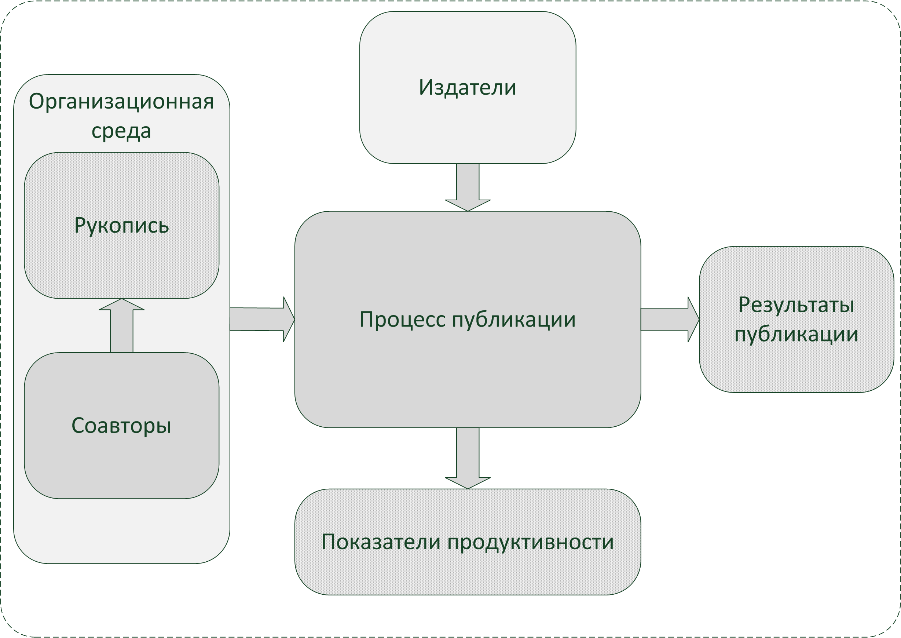
\includegraphics[width=0.8\textwidth]{om1}
  \label{fig:om1}
  \caption{Логический каркас исследования.}
\end{figure}  
Как видно из рисунка, логический каркас исследования включает в себя организационную среду (соавторы и их рукопись), процесс публикации, издателей, показатели продуктивности и результаты публикации.
В следующем подразделе каждый из компонентов логического каркаса будет рассмотрен подробнее.

\subsection{Рукопись}
Как упоминалось ранее, рукопись по форме - это текст.
Методологически рукописи разделяют на следующие основные виды:
\begin{itemize}
\tightlist
\item Монография
\item Научная статья
\item Тезисы доклада
\end{itemize}

Научная статья – это произведение небольшого объема, обычно от 5 до 20 страниц. По содержанию научные статьи разделяются на три типа: 
\begin{itemize}
\tightlist
\item Научно–теоретические статьи
\item Научно–практические статьи
\item Научно–методические статьи
\end{itemize}
Научно–практические статьи посвящены научным экспериментам и реальному опыту. 
Далее будет рассмотрен именно этот тип рукописей.

\subsection{Соавторы}
Большинство исследований выполняют научно-исследовательские коллективы, а не авторы-одиночки. Как следствие, рукописи тоже пишутся в результате коллективного труда. Согласно исследованию \cite{kradoya2016structure}, в нефтегазовой отрасли распределение количества соавторов имеет вид, представленный на рисунке (Рис. \ref{fig:om2}).

\begin{figure}[H]
  \centering
  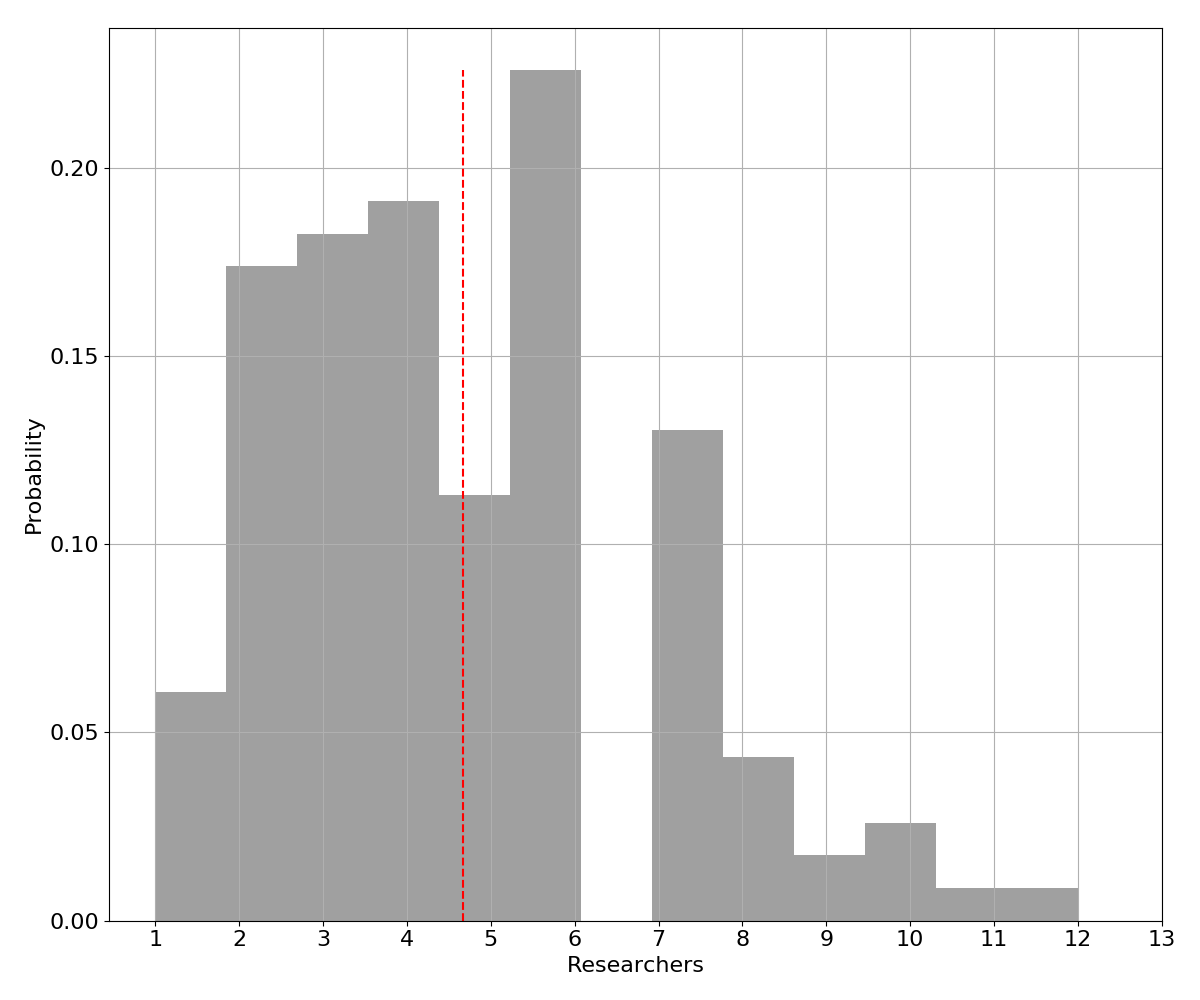
\includegraphics[width=0.8\textwidth]{om2}
  \label{fig:om2}
  \caption{Распределение количества соавторов научных статей в нефтегазовой отрасли. Красной линей обозначено среднее значение: 4.67. Стандартное отклонение распределения равно 2.28.}
\end{figure}  

\subsection{Организационная среда}
Научные исследования проводятся сотрудниками научно-исследовательских подразделений. 
В нефтегазовой отрасли такие подразделений могут принадлежать профильным институтам, научно-техническим центрам, сервисным организациям и другим участникам экосистемы. 
Таким образом, соавторы работают в организационной среде. 
Организационная среда во многом определяет коммуникации между соавторами, что важно на нашего исследования.

\subsection{Процесс публикации}
Процесс публикации состоит из двух типов действий: 
\begin{itemize}
\tightlist
\item Взаимодействие соавторов с издателем
\item Взаимодействие соавторов между собой
\end{itemize}

Объектом обоих действий является рукопись и сопутствующие дополнительные материалы: анкеты, презентации, письма, рецензии.
Основная задача взаимодействий с издателем состоит в удовлетворении условий для публикации статьи в данном издании. 
Обычно требования к авторам обозначены на веб сайтах издателей и могут отличаться.  
Взаимодействия соавторов между собой в процессе публикации включают следующие действия: 
\begin{itemize}
\tightlist
\item Формирование списка возможных издателей
\item Изучение специфики требуемых издателями тематик 
\item Определение временных ограничений на подачу рукописи
\item Составление плана доработок рукописи под требования издателей
\item Сбор сопутствующих документов по требованиям издателей
\item Подготовка презентации для доклада (обязательно для публикации в материалах конференций)
\item Выступление с докладом (командировка)
\item Подтверждение авторства в сообществах ученых и индексах.
\end{itemize}

\subsection{Издатели}
Наиболее значимыми считаются издатели, рекомендованные к публикации Высшей аттестационной комиссией (ВАК). В ``Перечне рецензируемых научных изданий'' ВАК по состоянию на 20.09.2017 содержится 2172 издания. 
Выберем издателей по одной, наиболее близкой для нефтегазовой отрасли специальности — 25.00 ``Науки о земле''. 
Таких изданий оказалось 147 штук. 
Далее автор разработал следующий алгоритм для сбора данных:

\begin{enumerate}
\tightlist
\item Осуществляем поиск веб сайта по названию издания
\item На сайте издания ищем раздел ``Для авторов''
\item Собираем перечень требований к рукописи и заносим в таблицу.
\item Переходим к следующему издателю.
\end{enumerate}

Воспользуемся результатами исследования \cite{mazov2015russian}, чтобы выбрать издателей с наибольшей публикационной активностью и импакт-фактором по международным реферативным базам. 
Список содержит 16 журналов. 
Все 16 журналов имеют общие правила для авторов, разработанные издательством МАИК ``Наука/Интерпериодика''.
Каждое издание имеет свой допустимый объём публикаций, обусловленный количеством статей в одном выпуске и количеством выпусков в год.
Чем больше рукописей поступает к издателю, тем выше конкуренция за право быть опубликованным.  

\subsection{Результаты публикации}
Результатом публикации является определенный вклад в науку. 
Задача максимизации доступности результатов исследования в эпоху Интернет может быть решена с помощью использования интернет ресурсов. 
Приведем лишь некоторые способы для увеличения аудитории: 

\begin{itemize}
\tightlist
\item Международные реферативные базы (Scopus, WoS), 
\item Электронные библиотеки (например, eLibrary.ru),
\item Присвоение научной статье идентификатора цифрового объекта (DOI), 
\item Привязка научной статьи к автору в онлайн сообществах ученых (например, ResearchGate),
\item Публикация статьи в открытых библиотеках (например, arxiv.org),
\item Привязка статьи к идентификационному номеру ученого (например, ORCID, SPIN),
\item Индексы цитирования (например, РИНЦ).
\end{itemize}

Индекс цитирования, например, Российский индекс научного цитирования (РИНЦ), является одним из распространенных наукометрических показателей и применяется для формальной оценки в научных кругах.
Альтернативами индексу цитирования являются экспертная оценка и оценка по импакт-фактору научных журналов.
Углубленные методы библиометрического анализа дают возможность рассмотреть вклад автора с различных точек зрения.
Большое внимание в частности уделяется анализу публикаций с помощью графов соавторства, рассмотренных далее в разделе \ref{sec:coath}. 
Пример графа соавторств приведен на рисунке (Рис. \ref{fig:om3}).

\begin{figure}[H]
  \centering
    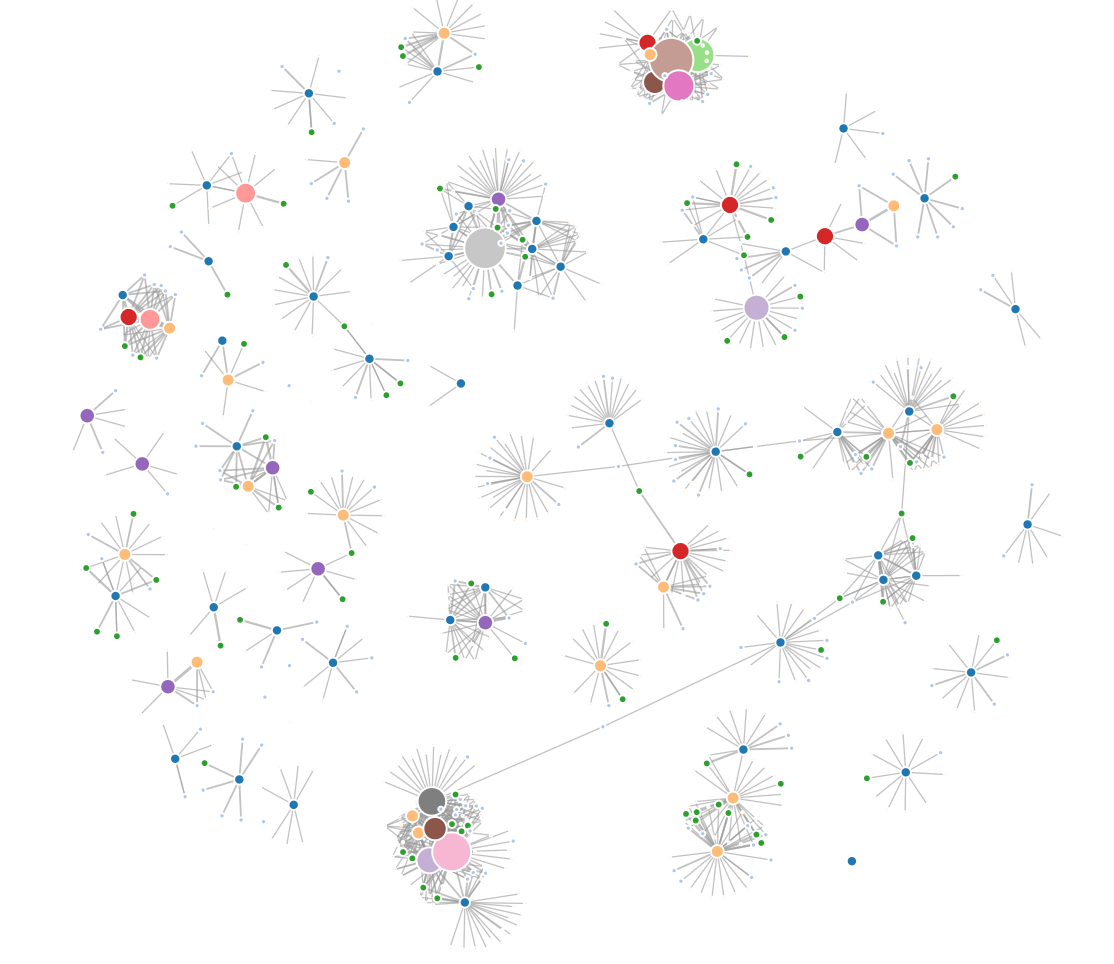
\includegraphics[width=0.8\textwidth]{om3}
  \label{fig:om3}
  \caption{Граф соавторств для ключевого слова \textit{Нефтяные оторочки}}
\end{figure}  

Графы соавторств позволяют визуально выделить наиболее значимых ученых по данной тематике. Например, на рисунке (Рис. \ref{fig:om4}) мы можем видеть такой кластер. 

\begin{figure}[H]
  \centering
    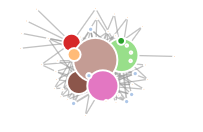
\includegraphics[width=0.2\textwidth]{om4}
  \label{fig:om4}
  \caption{Фрагмент графа соавторства по ключевому слову Нефтяные оторочки. Изображены только узлы, относящийся к профессору Rahim Masoudi.}
\end{figure} 

Принцип построения графов соавторств заключается в отнесении количества публикаций по выбранному ключевому слову к вершинам – авторам, а фактов соавторства к ребрам графа. 
Такой принцип построения графа позволяет анализировать его с помощью методов Анализа социальных сетей (Social network analysis, SNA).

\subsection{Показатели продуктивности публикаций}
Показатели продуктивности процесса публикаций должны давать интегральную характеристику процессу и позволять проводить сравнения различных реализаций процесса. Наиболее полезными представляется показатели, приведенные в таблице (Таб. \ref{tab:om1}):

\begin{table}[H]
\centering
\caption{Показатели продуктивности процесса публикаций}
\label{tab:om1}
\resizebox{\textwidth}{!}{%
\begin{tabular}{ |l|l| }
\hline
\textbf{Название показателя продуктивности} & \textbf{Описание} \\ \hline
Эффективность публикаций & Отношение количества опубликованных рукописей к общему количеству написанных рукописей \\ \hline
Доля опубликованных рукописей на одного автора & Отношение количества опубликованных рукописей к числу авторов \\ \hline
Доля отвергнутых издателями рукописей на одного автора & Отношение количества отвергнутых рукописей к числу авторов \\ \hline
\end{tabular}%
}
\end{table}

Предполагается, что процесс более продуктивен, когда \textit{Эффективность публикаций} стремится к единице, \textit{Доля опубликованных рукописей на одного автора повышается}, а \textit{Доля отвергнутых издателями рукописей на одного автора} стремится к нулю.
Стратегии управления процессом публикации через показатели продуктивности приведены в таблице (Таб. \ref{tab:om2}).

\begin{table}[H]
\centering
\caption{Стратегии управления продуктивностью процесса публикаций через показатели продуктивности.}
\label{tab:om2}
\resizebox{\textwidth}{!}{%
\begin{tabular}{ |l|l|l| }
\hline
\textbf{Название показателя продуктивности} & \textbf{Максимальная продуктивность} & \textbf{Минимальная продуктивность} \\ \hline
Эффективность публикаций & Стремится к единице & Стремится к нулю \\ \hline
Доля опубликованных рукописей на одного автора & Увеличивается & Уменьшается \\ \hline
Доля отвергнутых издателями рукописей на одного автора & Стремится к нулю & Увеличивается \\ \hline
\end{tabular}%
}
\end{table}
Отметим, что приведенные показатели продуктивности никак не характеризуют качество самой научной статьи.
В данном исследовании автор не ставит задачу оценки качества научной работы.

На основании вышеизложенных методических принципов может быть построена модель процесса с помощью системной динамики. 

\section{Теория суррогатного моделирования}

Суррогатная модель лежит в основе нового направления моделирования в инженерии.
Она является математическим методом составления модели, базирующейся на результатах испытаний и/или вычислительных экспериментов, проведенных с разнообразными объектами одного рассматриваемого класса.
В некоторых случаях суррогатное моделирование является единственным способом решения инженерно-технической задачи.

Задачей суррогатного моделирования является оптимизация исходной сложной функции таким образом, чтобы максимально уменьшить область расчета и свести его к минимуму. 
Для упрощения многих инженерных задач строится суррогатная модель целевой функции, которая впоследствии заменяет саму целевую функцию.

Концепция создания суррогатных моделей состоит из следующих этапов: 
\begin{itemize}
\tightlist
\item  
  Характеристика объекта Z, определяющая свойства объекта в некоторых условиях, может быть описана в виде функциональной зависимости $Z= \Phi(X,Y)$,  где переменная X описывает сам объект, а переменная Y задает условия функционирования.
\item
  Функция $\Phi$ является неизвестной, и для ее вычисления проводятся вычислительные эксперименты.
\item
  Имеется некоторое количество измерений $ \Xi = \{ X_i,Y_i,Z_i= \Phi_i ( X_i,Y_i ), i \in \mathbb{R} \} $,
где значение  $Z_i= \Phi_i (X_i,Y_i ) $ характеристики Z получено методом $M_i$ для объекта, имеющего описания $X_i$, в условиях функционирования $Y_i$.
\item
  По известному множеству $\Xi$ с помощью тех или иных математических методов анализа и обработки данных строится функция $\Phi^s (X,Y)$, значение которой принимаются в качестве приближенного значения характеристики Z для объекта с описанием X в условиях функционирования Y.

Если все значения в множестве $\Xi$ получены при помощи одной и той же модели $M$ и $\Phi^s (X,Y) = \Phi^m (X,Y)$, то построенная функция $\Phi^s$ может рассматриваться как ``заменитель'' (суррогат) функции $\Phi^m$.  
\end{itemize}

Суррогатное моделирование успешно применяется в таких областях как электротехника, нефтяное дело, водное хозяйство, военное дело, машиностроение и химическая отрасль.

Незаменимо применение суррогатных моделей и в строительстве для оптимизации аэродинамической формы для выявления оптимальной формы уникальных гражданских сооружений, таких как высотные здания и большепролетные мосты, которые окружены турбулентным потоком.

Следующие задачи нефтегазовой отрасли так же могут быть решены с использованием суррогатных моделей:

\begin{itemize}
\tightlist
\item Построение суррогатных модели резервуара (surrogate reservoir model);
\item Оптимизации расположения скважин;
\item Анализ неопределенности прогноза добычи нефти;
\item Автоадаптация модели резервуара по данным;
\item Задача оптимизации при суперэлементном моделировании разработки нефтяных месторождений.
\end{itemize}

В ряде вычислительных экспериментов для решения задач нефтегазовой отрасли используется вышеописанный мета-алгоритм. 
Например, сначала в гидродинамическом симуляторе производятся расчеты значения функции для определённых узловых значений параметров $X_i$ на основании физических законов движения жидкостей в пористой среде $M_i$, а потом, заданная таким числовым образом функция $\Phi$ используется для получения значений функции $Y_i$  либо на более детализированном множестве значений параметров, либо для значений параметров, выходящих за рамки узловых значений $X_i$.

Одна из основных причин возникновения описанного выше мета-алгоритма построение суррогатной модели заключаются в ограничениях на скорость гидродинамической моделирования. 
В будущем, когда в любое время любой специалист организации сможет варьировать значения параметров в широком диапазоне и в режиме близком к реальному времени получать искомые значения функции потребность в суррогатных моделях скорее всего отпадет.
А пока моделирование производится на дорогостоящих высокопроизводительных кластерах, специалистами за времена, измеряемые в часах, а иногда и днях для одного набора параметров существует потребность в прозорливой подготовке данных которые могут понадобиться в дальнейшем.
Так как, потребность в изменении параметров может возникать по несколько раз в день и у самых разных специалистов различных подразделений организации, то применение суррогатного моделирования является насущной необходимостью.
Получаемая суррогатная модель $\Phi^s$, иногда ее называют прокси-моделью, превосходит изначальную модель $\Phi^m$ по вычислительной силе во много раз, то есть, не требует большого объема вычислительных ресурсов и работает в режиме близком к реальному времени.

\section{Непараметрические модели}
Для того, чтобы понять, что такое непараметрические модели рассмотрим параметрические модели. 
Параметрической модель $p$ для значений $y$, зависящих от переменных $X$  и параметров $\theta$  будет иметь вид  $p \left( y\vert	,\theta \right)$.
Нахождение  параметров $\theta$ с помощью методов максимизации апостериорной вероятности $p \left( \theta \vert y,X \right)  \longrightarrow \max_\theta $.

Для поиска оптимальных параметров математической модели используются методы оптимизации.

Численные методы оптимизации:

\begin{itemize}
\tightlist
\item  Градиентные и безградиентные, 
\item  Одно и много критериальные, 
\item  Робастные (для задач оптимизации в условиях неопределенности), 
\item  Основанные на суррогатных моделях (surrogate -- based),
\end{itemize}

Рассмотрим методы Байесовской оптимизации, которые наиболее часто применяются в суррогатном и имитационном моделировании. 
При этом данные и модель являются ``черным ящиком''.

Пусть дана функция  $ f \left(  x \right)$  и нам нужно найти $x$ при котором она достигает максимума  $ f \left(  x \right) \longrightarrow \max_x$. Добавим условие при котором расчет каждого значения  $ f \left(  x \right)$ это ресурсоемкая задача. Такое условие встречается в следующих случаях: 

\begin{itemize}
\item $x$ - это географические координаты скважины, а  $ f \left(  x \right)$ -- это количество нефти, которое можно добыть, пробурив скважину с координатами $x$. В таком случае одно значение  $ f \left(  x \right)$ стоит миллионы рублей;
\item $x$ - это гиперпараметры искусственной нейронной сети глубокого обучения,  $ f \left(  x \right)$  -- это целевая метрика точности предсказания. В этом случае одно значение  $ f \left(  x \right)$ будет занимать месяцы работы;
\item $x$ - это лекарство, а  $ f \left(  x \right)$ - эффективность лекарства против болезни. В таком случае одно значение  $ f \left(  x \right)$ будет стоить жизни одного подопытного животного.
\end{itemize}

Таким образом, постановка задачи состоит в том, чтобы оптимизировать целевую функцию за минимальное количество попыток.
При этом использование суррогатных моделей целевой функции позволяет сделать каждый шаг оптимизации менее ресурсоемким. 
Введем функцию ценности обнаружения  $ \mu \left(  x \right)$, которая характеризует выгоду полученную от оптимизации  $ f \left(  x \right)$ при использовании суррогатной модели $\hat{f}$.
Функция ценности обнаружение является количественной оценочной функцией для минимализации количества попыток. 
Расмотрим следующие  $ \mu \left(  x \right)$:

\begin{itemize}
\item Maximum probability of improvement (MPI): $ \mu \left( x \right) = P(\hat{ f} \left( x  \right) \geq f^* + \epsilon =  \Phi \bigg( \frac{\mathbb{E}\hat{ f} \left( x  \right) - f^* -\epsilon}{Var[\hat{ f } \left( x  \right)]}\bigg) $, где $f^*$ - текущее лучшее значение.
\item Upper confidence bound (UCB): $  \mu \left(   x \right) = \mathbb{E}\hat{ f } \left( x  \right) + \eta Var[\hat{ f} \left( x  \right)] $
\item Expected improvement (EI): $  \mu \left(   x \right) = \mathbb{E} \max( f \left( x  \right) - f^*,0)  = Var[\hat( f \left( x  \right)] \cdot [z \Phi (z) + \phi(z)]$, где $z = \frac{\mathbb{E}\hat{ f }\left( x  \right) - m\left( x \right)}{Var[\hat{ f } \left( x  \right)]}$
\item 
\end{itemize}

\section {Байесовские методы для определения параметров НТЦ}

Рассмотрим результаты деятельности НТЦ как наблюдения $x$, тогда в самом общем смысле в качестве задачи поставим найти распределение случайной величины $\theta$, приводящей к имеющимся наблюдениям.

Согласно теореме Байеса имеем выражение \ref{eq:bay}.

\begin{equation} \label{eq:bay}
p \left(  \theta \vert x \right) = \frac{p \left ( x \vert \theta \right) \, p \left(  \theta \right)} {\sum_i p \left(  x \vert \theta_i \right) \, p \left(  \theta_i \right)}
\end{equation}

Для вычисления апостериорного распределения $p \left(  \theta \vert x \right)$ на основании функции правдоподобия $p \left ( x \vert \theta \right)$, априорного распределения с плотностью вероятности $p \left(  \theta_i \right)$ и полной вероятностью $p \left(  x \right) = \sum_i  p \left(  x \vert \theta_i \right) p \left(  \theta_i \right)$. 

Вычисление полной вероятности $p \left(  x \right)$ является сложной задачай, поэтому воспользуемся принципом максимизации апостериорной вероятности $p \left( \theta \vert  x \right)$. Найдем такие параметры $\theta_{MAP}$ при которых выражение $p \left( \theta \vert  x \right)$ максимально. Принцип максимализации апостериорной вероятности (Maximum A Posteriori, MAP) можно записать в виде: 
\begin{eqnarray*} 
\theta_{MAP} & = & \operatorname*{arg\,max}_\theta p \left( \theta \vert  x \right)\\
			 & = & \operatorname*{arg\,max}_\theta \frac{p \left( x \vert \theta \right) \, p \left( \theta \right)} {p \left(  x \right)}
\end{eqnarray*}

Так как полная вероятность $p \left(  x \right)$ не зависит от $\theta$, то можем убрать знаменатель и получить формулировку для оптимизационной проблемы в виде:
\begin{equation} \label{eq:mpopt}
\theta_{MAP} = \operatorname*{arg\,max}_\theta p \left( x \vert \theta \right) p \left( \theta \right)
\end{equation}

Уравнение ~\ref{eq:mpopt} не содержит $p \left(  x \right)$ и может быть решено с помощью численных методов. Но данный подход страдает от следующих проблем: 
\begin{itemize}
	\item Нет инвариантности относительно параметров распределения $\theta_{MAP}$;
	\item $\theta_{MAP}$ не применима в качестве априорного распределения;
	\item Нет возможности оценить байесовский достоверный интервал (credible interval).
\end{itemize}

Рассмотрим частный случай $\theta_{MAP}$ когда вероятности всех $\theta$ одинаковы - юниформное распределение. 
Тогда задача поиска $\theta$ сводится к поиску максимального значения для $p \left( x \vert \theta \right)$. 
Такой подход называют методом оценки максимального правдоподобия (maximum likelihood estimation, MLE).
Запишем выражение оптимизационной задачи для метода оценки максимального правдоподобия.

\begin{equation} \label{eq:mle0}
\theta_{MLE} = \operatorname*{arg\,max}_\theta p \left( x \vert \theta \right) = \operatorname*{arg\,max}_\theta \prod_i p \left( x_i \vert \theta \right)
\end{equation}

Без потери общности можем максимизировать логарифм от правой части выражения ~\ref{eq:mle0}.

\begin{equation} \label{eq:mle1}
\theta_{MLE} = \operatorname*{arg\,max}_\theta \log p \left(  x \vert \theta \right) 
\end{equation}

\begin{eqnarray*} \label{eq:mle2}
\theta_{MLE} & = & \operatorname*{arg\,max}_\theta \log \prod_i p \left( x_i \vert \theta \right) \\
             & = & \operatorname*{arg\,max}_\theta \sum_i \log p \left( x_i \vert \theta \right)
\end{eqnarray*}

Покажем подробнее как MAP преобразуется в MLE для случая юниформного распределения $\theta$:
\begin{eqnarray*} \label{eq:mapmle}
\theta_{MAP} & = &\operatorname*{arg\,max}_\theta \sum_i \log p \left( x_i \vert \theta \right) p \left( \theta \right) \\
             & = & \operatorname*{arg\,max}_\theta \sum_i \log p \left( x_i \vert \theta \right) \, const \\
             & = & \operatorname*{arg\,max}_\theta \sum_i \log p \left( x_i \vert \theta \right) \\
             & = & \theta_{MLE}
\end{eqnarray*}

Еще одним подходом к оценке $\theta$  является метод сопряжённых априорных распределений. 
В теореме Байеса ~\ref{eq:bay} изменяемым является только член $p \left( \theta \right)$, так как функция правдоподобия $p \left( x \vert \theta \right)$ определяется моделью, а $p \left(  x \right)$  данными.

Распределение априорной вероятности называется сопряженным с распределением постериорной вероятности, если они относятся к одному семейству распределений. 

Поясним вышеизложенное на примере. 
Пусть $p \left( x \vert \theta \right)$  и $p \left( \theta \right)$ являются нормальными распределениями.
Для распределения $p \left( \theta \right) = N(x \vert \mu_0,\sigma_0^2)$  с математическим ожиданием $\mu_0$ и дисперсией $\sigma_0^2$ выражение ~\ref{eq:bay} может быть записанно в виде ~\ref{eq:bayconj}.

\begin{equation} \label{eq:bayconj}
p \left( \theta \vert  x \right) = \frac{\mathbb{N}(x \vert \theta ) \, \mathbb{N}(\theta \vert \mu_0 , \sigma_0^2)} {p \left(  x \right)}
\end{equation}

Произведение двух нормальных распределений будет так же нормальным распределением, и параметры постериорного распределения можно будет вычислить по следующим формулам.
\begin{eqnarray}
\label{eq:bayconj1}
\mu & = & \frac{\left( \frac{\mu_0}{\sigma_0^2} + \frac{\sum_{i=1}^n x_i}{\sigma^2}\right)} { \frac{1}{\sigma_0^2}+ \frac{n}{\sigma^2} }\\
\sigma & = & \left( \frac{1}{\sigma_0^2} + \frac{n}{\sigma^2}\right)^{-1}
\end{eqnarray}

Таким образом использование сопряжённых семейств распределений позволяет избежать сложных вычислений полной вероятности.

\subsection{Скрытые параметры модели}
Говоря о характеристиках НТЦ, как объекта исследования мы не можем измерить такие параметры как интеллектуальный капитал (ИК).
Хотя ИК влияет на результаты деятельности НТЦ, которые мы можем измерить, например, на  количество публикаций и количество авторов.
Будем называть такие параметры как ИК скрытыми параметрами.

Для определения ИК можно рассмотреть подход на основании машинного обучения. 
Например, на основе искусственной нейронной сети. 
Тогда нам для обучения искусственной нейронной сети будет необходим набор данных, содержащий значения ИК для различных компаний с разными параметрами: количеством публикаций, количеством сотрудников, и.т.п.
Из литературы известно, что для обучения искусственных  нейронных сетей необходимы наборы данных с сотнями тысяч образцов и сотнями параметров.  
В действительности такого набора данных для НТЦ не существует. 
Но даже есть представить, что такой набор данных есть, то он будет содержать много пропущенных значений, противоречивых данных и других проблемных данных.

С другой стороны, Байесовская статистика может работать с небольшими наборами данных. 
Что приводит нас к рассмотрению вероятностного подхода к оценке скрытых параметров. 
Первым шагом для построений вероятностной модели является построение зависимости наблюдаемых параметров. И на первый взгляд все параметры будут зависит друг от друга. 
Например, чем больше авторов, тем больше публикаций, чем больше сотрудников с учеными степенями, тем больше публикаций в журналах из списка ВАК и т.п. 

%%Нужна картинка с картой связей без ИК. Каждый с каждым.

Но такая полносвязанная структура модели не позволяет нам построить структурированную вероятностную модель, так как нам необходимо будет оценить вероятность каждой возможной комбинации параметров.
А количество таких комбинаций будет экспоненциально расти с количеством рассматриваемых параметров.  

%%Нужна картинка с картой связей с ИК.
%% Bayesian network

Одним и решений может быть введение скрытых параметров, таких как ИК, которые уменьшают количество связей. 
Предположим, что НТЦ обладает ИК от которого зависит число публикаций и количество авторов. 
Таким образом, количество комбинаций для вероятностной оценки существенно сокращается.


\subsection{EM-алгоритм}
Рассмотрим вероятностную формулировку неравенства Йенсена. 
Пусть $(\Omega,\mathcal{F},\mathbb{P})$ — вероятностное пространство, и $X\colon\Omega \to \mathbb{R}$ — определённая на нём случайная величина. 
Пусть также $\varphi\colon\mathbb{R} \to \mathbb{R}$ — выпуклая (вниз) функция. 
Тогда, если $X, \varphi(X) \in L^1(\Omega,\mathcal{F},\mathbb{P})$, то  $\varphi(\mathbb{E}[X]) \leqslant \mathbb{E}[\varphi(X)]$, где $\mathbb{E}[\cdot]$ означает математическое ожидание. 
Или другими словами для выпуклой функции $f$ и распределения вероятностей $t$ получаем следующее выражение \ref{eq:jen}: 

\begin{equation} \label{eq:jen}
f (\mathbb{E}_{p \left( t \right)} \, t) \geqslant \mathbb{E}_{p \left( t \right)}f(t)
\end{equation}

Для дальнейшего рассмотрения приведем следующее определение расстояния Кульбака — Лейблера \ref{eq:kl0}. 

\begin{equation} \label{eq:kl0}
\mathcal{KL}(q \Vert  p) = \int_x q \left( x \right) \, \log \frac{q \left( x \right)}{p \left(  x \right)} \, {\rm d}x
\end{equation}

Отметим, что точнее будет называть расстояния Кульбака — Лейблера мерой различия двух распределений $q \left( x \right)$ и $p \left(  x \right)$, так как по определению данная мера не обладаем симметрией: $\mathcal{KL}(q \Vert p) \neq \mathcal{KL}(p \Vert q)$. 

Покажем еще одно полезное свойство расстояния Кульбака — Лейблера: $\mathcal{KL}(q \Vert p) \geqslant 0$.
Для этого произведем следующие вкладки:
\begin{eqnarray}\label{eq:kl03}
\mathcal{KL}(q \Vert   p) 
& = & \mathit{E}_q \left(  - \log	 \frac{q}{p} \right) \\
& = & \mathit{E}_q \left(  - \log	 \frac{p}{q} \right) \leqslant  \log \left( \mathit{E}_q \frac{q}{p} \right)\\
& = & \log \int_x q \left( x \right) \, \frac{q \left( x \right)}{p \left(  x \right)} \, {\rm d}x \\
& = & 0
\end{eqnarray}
Рассмотрим применение EM-алгоритма для нахождения скрытых параметров НТЦ.
Предположим, что у на есть модель НТЦ со скрытыми параметрами. 
Обозначим скрытые параметры как $t_i$, а наблюдаемые параметры как $x_i$. 
Тогда функцию правдоподобия можно выразить как ~\ref{eq:em0}.
\begin{equation} \label{eq:em0}
p \left( x_i \vert	\theta \right) = \sum_c p \left( x_i \vert t_i = c \right) p \left( t_i = c \vert \theta \right) 
\end{equation}

Где $p \left( t_i = c \vert \theta \right)$  - это априорная вероятность того, что $t$ принимает значение $t$. 
Задача состоит в том, чтобы максимизировать вероятность функции правдоподобия по $\theta$. 
Так как логарифм является выпуклой непрерывно возрастающей функцией, то будем искать максимум логарифма от $p \left( x_i \vert	\theta \right)$. 
Предположим так же, что все $N$ измерений $x_i$ были сделаны независимо. 
Тогда вероятность $X = \prod_i^N p \left( x_ \vert \theta \right) $

\begin{equation} \label{eq:em1}
\log p \left(  X \vert	\theta \right) = \sum_i^N \log p \left( x_i \vert \theta \right) = \sum_i^N \log \sum_c p \left(  x_i \vert t_i = c \vert \theta \right)
\end{equation}
Стоит отметить, что мы можем искать максимум выражения ~\ref{eq:em1}  с помощью градиентных методов. 
Например, с помощью метода стохастического градиентного спуска. 
Но автор сознательно применил другой алгоритм и покажет его преимущества далее.

Применим неравенства Йенсена ~\ref{eq:jen} к выражению ~\ref{eq:em1} и получим $\log p \left(  X \vert	\theta \right) \geqslant \mathfrak{L}(\theta, q)$.  
Далее выберем функцию $\mathfrak{L}(\theta, q)$ так, чтобы ее легко было максимизировать.
\begin{equation} \label{eq:em2}
\mathfrak{L}(\theta, q) = \sum_i^N \sum_c q(t_i = c) \log \frac{p \left( x_i, t_i = c \vert \theta \right)}{q(t_i = c)}
\end{equation}
И в итоге для параметра $\theta$ и распределения $q$ получим неравенство ~\ref{eq:em3}:
\begin{equation} \label{eq:em3}
\log p \left(  X \vert	\theta \right) \geqslant \mathfrak{L}(\theta, q)
\end{equation}
Теперь для поиска максимума $mathfrak{L}(\theta, q)$  применим  следующий итерационный алгоритм из двух шагов для каждой итерации $k$:

\begin{itemize}
	\item Фиксируем $\theta^k$ и выбираем $q^k$ так чтобы $\mathfrak{L}(\theta^k, q^k)$ была максимальной
	\item Получаем $q^{k+1} = \operatorname*{arg\,max}_q \mathfrak{L}(\theta^k, q)$
\end{itemize}

Первый шаг принято называть E-шаг, а второй M-шаг. Вместе они представляют EM-алгоритм результатом, которого является $\theta$ для скрытой переменной $t$. 

\subsection{E-шаг}
Рассмотрим более подробно E-шаг. 
Максимизация функции нижней границы $\mathfrak{L}(\theta^k, q^k)$ означает, что расстояние между $\mathfrak{L}(\theta^k, q^k)$ и функцией максимального правдоподобия $\log p \left(  X \vert	\theta^k \right)$. 
Запишем это уравнение для k-й итерации и покажем, что это расстояние можно выразить через расстояния Кульбака — Лейблера.
\begin{eqnarray*} \label{eq:em4}
DIST & = & \log p \left( X \vert \theta \right) - mathfrak{L}(\theta, q) \\
       & = & \sum_i^N \log p \left( x_i,\theta \right) - \sum_i^N \sum_c q(t_i = c) \log \frac{p \left( x_i,t_i=c \vert \theta \right)}{q(t_i=c)} \\
       & = & \sum_i^N  \big\{ \log p \left( x_i \vert \theta \right) \sum_c q(t_i=c) - \sum_c q(t_i = c) \log \frac{p \left( x_i,t_i=c \vert \theta \right)}{q(t_i=c)} \big\} \\
       & = & \sum_i^N \sum_c q(t_i = c) \big\{ \log p \left( x_i \vert \theta \right) - \log \frac{p \left( x_i,t_i=c \vert \theta \right)}{q(t_i=c)} \big\} \\
       & = & \sum_i^N \sum_c q(t_i = c) \big\{ \log p \left( x_i \vert \theta \right) - \log \frac{p \left( x_i,t_i=c \vert \theta \right)}{q(t_i=c)} \big\} \\
       & = & \sum_i^N \sum_c q(t_i = c) \log  \frac{p \left( x_i \vert \theta \right) q(t_i=c)}{p \left( x_i,t_i=c \vert \theta \right)}  \\
       & = & \sum_i^N \sum_c q(t_i = c) \log  \frac{p \left( x_i \vert \theta \right) q(t_i=c)}{p \left( t_i \vert x_i,\theta \right) p \left( x_i \vert \theta \right)}  \\
       & = & \sum_i^N \sum_c q(t_i = c) \log  \frac{ q(t_i=c)}{p \left( t_i \vert x_i,\theta \right) }  \\
       & = & \sum_i^N \mathcal{KL}( q(t_i)  \Vert   p \left( t_i \vert x_i, \theta \right) )\\
\end{eqnarray*}

Таким образом, максимизация функции нижней границы $\mathfrak{L}(\theta^k, q^k)$ эквивалентна минимизации суммы расстояний Кульбака — Лейблера для $q(t)$ и $p \left( t \vert x, \theta \right)$. 
Так как расстояния Кульбака — Лейблера неотрицательны по определению, то мы можем приравнять их нулю для поиска глобального минимума.
\begin{equation} \label{eq:em5}
0 = \sum_i^N \mathcal{KL}( q(t_i)  \Vert   p \left( t_i \vert x_i, \theta \right) ) 
\end{equation}

Также из определения расстояния Кульбака — Лейблера известно, оно равно нулю только в случае если оба распределения совпадают. 
\begin{equation} \label{eq:em6}
 q(t_i)  =  p \left( t_i \vert x_i, \theta \right) 
\end{equation}
Уравнение ~\ref{eq:em6}  означает, что для нахождения оптимального распределения $q(t)$ мы должны выбрать его равным постериорному распределению $p \left( t \vert x,\theta \right)$.

\subsection{М-шаг}
На М-шаге производится максимизация функции правдоподобия ~\ref{eq:em2} при фиксированном $q(t)$ по $\theta$.
\begin{eqnarray*} \label{eq:em7}
\mathfrak{L}(\theta, q) & = &  \sum_i^N \sum_c q(t_i = c) \log \frac{p \left( x_i, t_i = c \vert \theta \right)}{q(t_i = c)} \\
& = &  \sum_i^N \sum_c q(t_i = c) \log p \left( x_i, t_i = c \vert \theta \right) - \sum_i^N \sum_c q(t_i = c) \log {q(t_i = c)} 
\end{eqnarray*}

Отметим, что так как выражение $\sum_i^N \sum_c q(t_i = c) \log  {q(t_i = c)}$ не зависит от $\theta$, то при дифференцировании оно обнулится. 
Таким образом, выражение ~\ref{eq:em7}  можно преобразовать следующим образом.
\begin{equation} \label{eq:em8}
\mathfrak{L}(\theta, q)  = \mathbb{E}_{q}\log p \left( X,T \vert \theta \right) + const
\end{equation}

Напомним, что в выражении ~\ref{eq:em8} $X$ - это все данные, а $T$ - это все значения скрытых переменных. $\mathbb{E}_{q}$ обозначает математическое ожидание распределения $q$. Так как мы выбираем распределения для $X$ и $T$, то в наших силах обеспечить чтобы $ p \left( X,T \vert \theta \right)$ была гладкой и непрерывной. Такой выбор значительно упростит нахождения экстремума по $\theta$.

\subsection{Сходимость ЕМ-алгоритма}
ЕМ-алгоритм предназначен для нахождения локальных экстремумов функции максимального правдоподобия. 
Для этого используется функция нижней границы $\mathfrak{L}(\theta^k, q^k)$, которая в процессе оптимизации не убывает ~\ref{eq:em9}. 
\begin{equation} \label{eq:em9}
\log p (X \vert  \theta ^{k+1} ) \geqslant \log p (X \vert  \theta ^{k} )
\end{equation}

\subsection{Использование ЕМ-алгоритма для выявления скрытых тематик в тексте}
Научный текст является одним из проявлений деятельности НТЦ. 
Выявление тематик текста может быть сделано с использованием распределения Дирихле. 
Байесовская модель для постериорного распределения скрытых тематик в тексте может быть записана в следующем виде.

\begin{eqnarray*} \label{eq:lda1}
p \left( W,Z,\Theta \right) = \prod_{d=1}^{D} p \left( \theta_d \right) \prod_{n=1}^{N_d} p \left( z_{dn} \vert \theta_d \right) p \left( w_{dn} \vert z_{dn} \right) \\
p \left( \theta_d \right) \sim Dir( \alpha ) \\
p \left( z_{dn} \vert \theta_d \right) = \theta_{dz_{dn}} \\
p \left( w_{dn} \vert z_{dn} \right) = \Phi_{z_{dn}w_{dn}} \\
\sum_w \Phi_{tw} = 1 \\
\Phi_{tw} \geqslant 0
\end{eqnarray*}

Таким образом, что $W$ - это текстовые данные (научные статьи, документы),  $\Phi$ - распределение слов в каждой тематике, $Z$ - распределение тематик для каждого слова, $\Theta$ - распределение тематик в документе.
Оптимизационная задача для поиска тематик выглядит следующим образом: 
\begin{equation} \label{eq:lda2}
P(W \vert \Phi) \rightarrow max_\Phi
\end{equation}

Для использования ЕМ-алгоритма выпишем явно уравнения для Е-шага и М-шага:

Е-шаг:
\begin{equation}\label{eq:lda3}
\mathcal{KL} (q(\Theta) \, q(Z)  \Vert   p \left( \Theta,Z \vert W \right) ) \rightarrow \underset{q(\Theta) \, q(Z)} {\text{minimize}}
\end{equation}

М-шаг:
\begin{equation}\label{eq:lda4}
\mathbb{E}_{q(\Theta) \, q(Z)} \log p \left( \Theta,Z,W \right) \rightarrow \underset{\Phi}{\text{maximize}}
\end{equation}

Полученные выражения для Е-шага (\ref{eq:lda3}) и М-шага (\ref{eq:lda4}) позволяют получить скрытые тематики их текста. 

\section{Моделирование самоорганизующихся команд в научной среде}

Самоорганизация рабочих групп представляет большой интерес для научно-технических организаций, ищущих новые формы эффективной организации труда сотрудников.
Рассмотрение феномена самоорганизации, как альтернативы формированию рабочих групп привело к построению модели процесса самоорганизации. 
Рассмотрение жизненного цикла рабочей группы по отношению к поставленной цели позволило ввести формальные критерии оценки эффективности работы группы и прогнозировать ее продуктивность.

Важным фактором, влияющим на продуктивности рабочей группы, является характер решаемой задачи. 
Автор предложил собственную классификацию творческих задач нефтегазовой отрасли на основании компетенций, необходимых для их решения. 

В рамках разработанной методики жизненного цикла рабочей группы и классификации задач была построена математическая модель самоорганизации рабочих групп для решения творческих задач. Калибровка математической модели появления рабочих групп была проведена на данных Газпромнефть НТЦ. 

В созданной системе показателей эффективности был проведен цифровой имитационный эксперимент для выявления основных характеристик самоорганизации рабочих групп.

В результате была сделана кластеризация творческих задач по эффективности решения различными рабочими группами, составлены рекомендации по созданию организационных мероприятий, способствующих повышению вероятности самоорганизации рабочих групп, выделены критерии отнесения творческих задач к различным типам рабочих групп, определены основные критерии для формирования эффективных рабочих групп.

Моделирование групповых действий индивидуумов зависит от потенциальных участников группы и целей. 
Например, фанаты футбольного клуба легко объединяются в группу, но не имеют конкретной цели. 
С другой стороны, ученые могут объединяться в исследовательскую группу для конкретной цели, например, написания научной статьи. 
Одинаковы ли принципы объединения в этих случаях? 

Разделяют два процесса появления групп:
\begin{enumerate}
\item Самоорганизация – процесс упорядочения сотрудников за счёт внутренних факторов, без внешнего специфического воздействия, 
\item Формирование – назначение участников группы из вне.
\end{enumerate}

Пример формирования группы в организационной среде: 

\textit{Начальник управления принимает решение сформировать рабочую группу для создания системы разработки месторождения из двух разработчиков месторождений}. 

Пример самоорганизации группы в организационной среде: 

\textit{Несколько разработчиков месторождений решили, что им вместе нужно усовершенствовать методы обработки данных о технических режимах работы скважин с помощью методов машинного обучения и самозабвенно работают в вместе по выходным над этой задачей.
} \label{exp:2}

Решение о создании группы внутри ведет к самоорганизации, решение о создании группы из вне формирует группу. 
Отметим, что на практике процесс появления рабочих групп представляет суперпозицию самоорганизации и формирования. 
Но для исследовательских целей в данной работе авторы намерено рассматривают формирование и самоорганизацию раздельно для выявления родовых признаков этих явлений.

Группа создается на определенное время и для решения конкретной задачи. 
В этом смысле на лицо признаки проектной деятельности – уникальность результата и ограниченность ресурсов для достижения поставленной цели. 
Таким образом, обоснованным представляется применять проектную методику оценки эффективности группы, как проектной команды. 

Структура группы определяется характером решаемых задач. 
Для задач массового обслуживания, например, в рабочие группы в центрах обработки вызовов объединяют специалистов с определенным, одинаковым профилем компетенций. 
Разделение обязанностей в такой группе почти нет: типовые задачи по обслуживанию требуют стандартизованных действий членов группы.
Нагрузка равномерно распределяются по членам группы.

Группа, созданная для решения творческой задачи менее однородна. 
Для решения творческой задачи необходимы специалисты с разными компетенциями. 
Образно можно представить, как задача декомпозируется на компетенции участников.
И это не равномерное распределение, участникам достаются разные объемы работы в рамках их компетенций. 
Для приведенного выше примера (Пример  \ref{exp:2}), задача требует компетенций в технических режимах работы скважин и методах машинного обучения. 
Что будет, если компетенций нужных для достижения цели нужно больше, чем есть у группы? 
Каждый из участников группы выполнит работы в рамках своих компетенций, но цель не будет достигнута, так как останутся невыполненные работы. 
Это распространенная ситуация, как при неправильном планировании групп (формировании), так и при самоорганизации групп. 
Результат работы в такой ситуации оказывается отрицательным, но отношение к этому результату разное в случае самоорганизации и формирования.

Основными критериями эффективности рабочих групп является результат их деятельности и сроки достижения этого результата – это общепринятые организационные показатели эффективности.
Исследование феномена самоорганизации рабочих групп в динамике является сложнейшей организационной задачей. 
Поэтому автор использовал в данной работе математическую модель феномена самоорганизации рабочих групп. 
Математическая модель дает возможность изучить наиболее характерные аспекты феномена самоорганизации, но обладает определённой степенью приближения, неточности. 
Вычислительный эксперимент на основании созданной модели самоорганизации рабочих групп, который представлен далее состоит в том, чтобы оценить результаты работы различных групп над различными задачами. 
В связи с такой постановкой эксперимента возникают следующие исследовательские вопросы: 
\begin{enumerate}
\item Как происходит самоорганизация групп? Какие сотрудники могут самоорганизоваться, а какие нет? Как на самоорганизацию влияют компетенции, опыт, социальные факторы?
\item Какие организационные условия необходимы для самоорганизации групп в научно-технической среде? Конкурсы? Обучения? Мероприятия? 
\item С каким типом задач самоорганизованные группы справляются эффективнее, чем сформированные? 
\item Каковы принципы формирования групп для наиболее эффективного решения творческих задач? 
\end{enumerate}

Оценке эффективности научно-исследовательских и опытно-конструкторских проектов, а также исследованию факторов, влияющих на результативность научной деятельности посвящены многочисленные публикации, см., например, \cite{shcherb1982,ovch2009,fursov2016,shmatko2017}.
Как правило, в этих работах научный коллектив рассматривается как ``чёрный ящик'', производящий научные результаты, и оценка его эффективности производится только на основе выпускаемых результатов, внутренняя структура исследовательской группы обычно не берется в учёт. 
Самоорганизующиеся команды подробно изучены в работе \cite{moe2008understanding}.  
Отдельно исследуются мотивирующие факторы \cite{shmatko2017} и факторы, влияющие на результативность \cite{fursov2016}.

При этом тема моделирования и анализа командной работы также является хорошо проработанной и активно исследуется с середины XX века, см. \cite{bavelas1948mathematical,nov2008,bei2014}. 
Формальное описание профиля компетенций --- это тема многочисленных исследований и публикаций, см., например, \cite{rozewski2009competence,bei2014}.

Первым приближением может быть модель ограниченная существованием фиксированного набора определенных навыков. 
При этом профиль компетенции каждого сотрудника можно описать в виде вектора значений, в котором каждая координата описывает уровень его владения соответствующим навыком.

Вектор, описывающий профиль компетенций команды, получается в результате простого сложения профилей компетенций участников. 
Такая модель естественно возникает, если измерять уровень компетенции производительностью при выполнении соответствующего типа задач. 
Тогда естественно предполагать, что при совместной работе в команде производительность участников складывается.

Аналогичным вектором можно также описать и профиль задачи.
Для подготовки и проведения научного исследования с учетом ограничения по времени требуется определенный уровень производительности для каждого типа задач.

В данной работе рассматриваются самоорганизующиеся малые команды, в которых инициатива создания исходит от сотрудников. 
Это допущение соответствует реальной ситуации в большинстве научных коллективов, где администрация может различными способами мотивировать сотрудников подать заявку на участие в той или иной научной конференции или рекомендовать подготовить статью для определенного журнала, но итоговое решение, как правило, остается за научным сотрудником.

В данной работе предполагается, что список компетенций и уровень опыта  являются критериями, на основе которого сотрудник принимает решение о присоединении к команде.

В качестве входных данных модели рассматривается набор тематик, которые соответствуют последовательности поступающих приглашений от конференций и журналов, в которые открыт прием заявок. 
Для каждого мероприятия или издания известна одна или несколько тем. 
Подготовка статьи по заданной тематике требует определенного набора компетенций. 

Компетенции определяются пространством научной деятельности. В нефтесервисной индустрии набор компетенций отличается от набора компетенций в деревообрабатывающей индустрии. 

Опыт описывает вектор определенной длинны и направления в пространстве компетенций. 
Проекции вектора опыта на оси компетенций показывают опыт в соответствующей компетенции. 

Задача, например тема научной статьи, так же представляет вектор в пространстве компетенций. 
Темы могут требовать компетенций, которыми не обладают авторы по отдельности. 
Каждый соавтор закрывает только часть требуемых для решений задачи (написания статьи) компетенций.  

\subsection{Старт процесса командообразования}

Процесс образования команды начинается с принятия первым участником решения о создании команды для подготовки заявки на конференцию или статьи в сборник.
Происходит это следующим образом. 
Незанятый сотрудник просматривает список приглашений и производит оценку своих компетенций с точки зрения объявленных тематик. 
Если хотя бы одна из его компетенций соответствует или превосходит требования цели, он принимает решение о создании команды и становится первым ее участником.
В начальный момент профиль компетенций команды совпадает с профилем первого участника.
Следующие участники будут присоединяться к этой команде учитывая  требования, соответсвующие выбранной тематике, а так же профили компетенций других членов команды. 

\subsection{Присоединение новых участников к команде}

Второй (последующий) участник узнает от одного из членов команды о цели и оценке текущих компетенций команды. 
Эта информация распространяется между сотрудниками, которые достаточно хорошо знакомы друг с другом. 
В модели это представлено с помощью коммуникационного графа. 
Каждый последующий участник производит оценку своих компетенций с точки зрения потребностей команды для достижения цели и принимает решение о присоединении к команде. 
Решение положительно, если хотя бы одна из компетенций этого участника при добавлении к профилю команды приближает ее к поставленной цели.

\subsection{Финализация состава команды}

В виду ограниченности  времени на решение поставленной задачи, время на формирование команд тоже не может быть безграничным.
Если в течение отведенного отрезка времени команду с требуемым набором компетенций сформировать не удалось, процесс останавливается, участники освобождаются от принятых обязательств и переключаются на поиск другой задачи. 
Если же команда успешно сформирована, то считаем, что входящие в нее сотрудники заняты некоторое время и итогом этой работы является публикация.

\subsection{Формальная модель компетенций}

Пусть $N$ обозначает количество ключевых навыков, которые необходимы для работы в данной предметной области, $W$ - множество сотрудников организации. 
Тогда профилем компетенций для сотрудника называется вектор $\vec{\kappa} \left( w \right)$ (\ref{eq:team1}).

\begin{equation}\label{eq:team1}
\vec{\kappa}\left( w \right) = (\kappa_1, \ldots, \kappa_{\bf N}) \mbox{, где } w\in {W}, \kappa_i \in \mathbf{R}^{+}.
\end{equation}

Профиль компетенций команды $T$ состоящей из $M$ человек - это вектор той же размерности $N$, который определяется как сумма по всем участникам команды:

\begin{equation}\label{eq:team2}
\vec{\kappa} \left( T \right)  = \sum_{i=1}^{{\bf M}}
\vec{\kappa} \left( w_i \right) \mbox{, где } 
T= \{w_1, \ldots, w_{\bf M} : w_i \in {W} \}.
\end{equation}

Неформально $i$-я компонента вектора соответствует производительности человека и команды при выполнении задач определенного типа.
Профиль тематики $p$ имеет тот же тип, а именно является $N$-мерным вектором:
\begin{equation}\label{eq:team3}
\vec{\kappa}(p) = (\kappa_1, \ldots, \kappa_N).
\end{equation}

Тут $i$-я компонента вектора соответствует минимальной производительности команды, при которой все задачи соответствующего типа будут выполнены гарантировано в срок и с надлежащим качеством.

\subsection{Модель принятия ключевых решений}

Для реализации процесса командообразования ключевыми являются функции, моделирующие логику принятия решения на разных этапах формирования команды, а именно:
\begin{itemize}
\item $\alpha(w, p)$ описывает выбор цели первым участником команды, а именно $\alpha(w, p)=1$ если сотрудник $w$ рассматривая цель $p$ принимает положительное решение о создании команды и $\alpha(w, p)=0$ в противном случае; 
\item $\beta(w, T, p)$ формализует принятие решения о присоединении к команде вторым и последующими участниками;
\item $\gamma(T, p, t)$ моделируют решения  о самороспуске в момент времени t на основании сопоставления профиля созданной команды и профиля задачи. 
\end{itemize}

В данном исследовании предполагается, что $\alpha$, $\beta$ и $\gamma$ являются детерминированными булевозначными функциями, которые зависят только от профиля компетенций человека, команды и задачи соответственно. 

\begin{eqnarray} \label{eq:team4}
\alpha(w, p) = \alpha'(\vec{\kappa}(w), \vec{\kappa}(p)),\\
\beta(w, T, p) = \beta'(\vec{\kappa}(w), \vec{\kappa}(T), \vec{\kappa}(p)),\\
\gamma(T, p, t) = \gamma'(\vec{\kappa}(T), \vec{\kappa}(p), t).
\end{eqnarray}

Пусть далее $\bf K$ обозначает всё пространство возможных значений вектора компетенций. Тогда тот факт, что в нашей модели алгоритм командообразования зависит только от профилей компетенций участника, команды и цели, задает тип функций $\alpha'$, $\beta'$ и $\gamma'$:

\begin{eqnarray} \label{eq:team5}
\alpha': {\bf K} ^2 \to \{0, 1\},\;\;\;
\beta': {\bf K} ^3 \to \{0, 1\},\;\;\;
\gamma': {\bf K} ^2 \to \{0, 1\}
\end{eqnarray}

Эти функции можно описать в виде следующих логических формул:

\begin{eqnarray} \label{eq:team6}
\alpha'(x,y)=1 \iff \exists i (x_i \geq y_i) \\
\beta'(x,y,z)=1 \iff \exists i [(x_i > y_i) \wedge (y_i < z_i)]  \\
\gamma'(x,y,t)=1 \iff \exists i (x_i < y_i)  \wedge (t > \tau_{\max})
\end{eqnarray}

\subsection{Процесс формирования команды}
На момент командообразования фиксирован список открытых задач ${P}$ и для каждой конкретной задачи $p\in {P}$ задан её профиль $\kappa(p)$. 
Также фиксировано множество сотрудников $W$ и для каждого сотрудника $w\in W$ известен профиль его компетенций $\kappa(w)$. 
Кроме этого задан граф коммуникаций между сотрудниками $G\subseteq W\times W$. 
Ещё одним параметром является время $\tau_{\max}$ в течение которого команда должна сформироваться.

На каждом шаге последовательно происходит следующее.
\begin{enumerate}
\item 
Каждый сотрудник $w_0$, который не включен ни в одну из команд и не получил приглашение о вступлении в команду рассматривает список целей $P$. В случае если находится $p_0$ для которой $\alpha(w_0,p_0)=1$, сотрудник принимает решение о создании новой команды $T_0$ и отправляет приглашения присоединиться к команде всем соседям в коммуникационном графе $G$.

\item Если сотудник $w_1$ не был включен в команду и получил приглашение войти в команду $T_1$, созданную для решения задачи $p_1$, он принимает приглашение, если $\beta(w_1,T_1,p_1) = 1$ и отправляет приглашения всем своим соседям в графе $G$. В противном случае приглашение отклоняется.

\item Если для какой-то команды $T_2$, созданной для решения задачи $p_2$, выполняется условие $\gamma(T_2,p_2)=1$, команда приступает к работе и все приглашения аннулируются.

\item Если для какой-то команды $T_3$, созданной для решения задачи $p_3$, спустя заданное время $\tau_{\max}$ выполняется условие $\gamma(T_3,p_3)=0$, эта команда расформировывается и все приглашения аннулируются.

\end{enumerate}

Несмотря на то, что что $\alpha$, $\beta$ и $\gamma$ являются детерминированными, алгоритм допускает большую степень неопределенности, которая связана с недетерминированным характером взаимодействия объектов внутри системы. 
В частности, на результат существенно влияют следующие параметры, которые реализуются вероятностно:
\begin{itemize}
\item очередность рассмотрения списка задач свободным сотрудником;
\item очередность рассмотрения сотрудником полученных приглашений;
\item очередность, в которой выбираются сотрудники для применения очередного шага алгоритма. 
\end{itemize}

Построенная модель является основой для дальнейших исследований процесса образования и функционирования проектных команд в научной среде. 
В частности, на её основе планируется разработать методику оценки эффективности научно-исследовательской деятельности.
Также интересным направлением работы является уточнение и расширение модели, в частности:

\begin{itemize}
\item 
Модели компетенций могут быть уточнены с привлечением аппарата нечёткой логики.
\item 
При моделировании долгосрочных периодов появляется необходимость учитывать профессиональное и карьерное развитие сотрудников и сопряженные с этим изменения в их профилях компетенций. 
\item 
Функции $\alpha$, $\beta$ и $\gamma$, описывающие процесс принятия ключевых решений, могут быть уточнены путем учёта других индивидуальных и командных характеристик, а также специфики задач.
\item 
Алгоритм командообразования может иметь более сложную итеративную логику, учитывающую различные подходы к гибкому управлению проектами.
\item 
Отдельной проработки заслуживает ситуация с неуспешным завершением проекта. 
В терминах научной деятельности это означает, что написанная публикация не была принята к печати, но полученные результаты являются хорошим заделом для дальнейшей работы. 
В текущей работе автор сделал допущение, что сотрудники не пишут \textit{в стол}, а каждое соавторство ведет к публикации.
\end{itemize}

\section{Методика графа соавторства}
\label{sec:coath}
Сложившаяся практика построения графов соавторства подразумевает использование математического аппарата теории графов. Традиционно для построения графов соавторства используют неориентированные графы.
Граф соавторства представляет наглядную визуализацию выбранного научного сообщества и позволяет производить анализ с помощью таких распространенных метрик графов, как: Betweenness centrality \cite{leifeld2017collaboration,koseoglu2018authorship,ho2017basic} и Closeness centrality \cite{chang2017hidden,paraschiv2017semantic,ahmed2017analysis}. Данные метрики, как и метрика Degree, предназначены для формального выделения важных вершин графа.

\subsection{Двудольные графы}
Существенным аспектом для построения графа соавторств является выборка данных для анализа. 
Обычно исследователи используют публичную библиографическую информацию, содержащую список соавторов. 
Источником такой информации может быть Google Scholar, ArXiv и другие онлайн библиотеки. 
Рассмотрение открытых научных сообществ так же интересно, как и сужение выборки до одной страны \cite{krasnov2013measurement}, отрасли \cite{gielfi2017university} и даже организации \cite{kradoya2016structure}.
Добавление в граф полей, связанных с аффиляцией автора, позволяет сделать исследования отношения организаций.
Как пример, в работе \cite{gielfi2017university} авторы анализируют связи между исследовательскими институтами и индустриальными научными центрами в нефтегазовой индустрии.
Такой подход к выборке позволяет проанализировать топологию связей между организациями, на основании принадлежности авторов к организации. 

Отметим, что все приведенные выше исследования не принимают в расчет содержание исследовательских статей.
Эта особенность будет важна в дальнейшем. 
Среднее количество соавторов может изменяться в зависимости от индустрии, но в целом количество соавторов растет.
Отметим этот факт, как структурную особенность исследуемой области. 

В приведенных выше исследования граф соавторства строится на неориентированный граф.
Авторы равнозначны в соавторстве, хотя на деле это не так. 
В работе автора \cite{krasnov2017model} проанализирована структура команды соавторов и сформулированы возможные роли в процессе исследования. 

Кроме того, в традиционном построении графа соавторства информация о всех совместных исследовательских работа содержится в ребрах графа. 
Часто ребра рисуют различной толщины или цвета в зависимости от количества совместных работ, но данная характеристика ребер не рассматривается в контексте метрик графа, так как не отражает коммуникационный смысл повторного соавторства.
С учетом этих ограничений сформулируем следующий исследовательские вопросы: 

\begin{que}[И.В.\ref{que:ex1}] 
\label{que:ex1}
Существуют ли другие способы построения графа соавторств? 
\end{que}

\begin{que}[И.В.\ref{que:ex2}] 
\label{que:ex2}
Какими преимуществами и недостатками обладают различные способы построения графа соавторств? 
\end{que}

\begin{que}[И.В.\ref{que:ex3}]
\label{que:ex3}
Каковы количественные, сравнимые характеристики графов соавторств? 
\end{que}

В приведенных выше исследованиях граф соавторства строится как неориентированный граф: статьи становятся равнозначными ребрами, соединяющими авторов. 
Автор данного исследования считает, что более информативным будет построение графа соавторств как двудольного графа. 
Такой подход позволяет включить в граф соавторств информацию о научных статьях. 
На Рисунке \ref{fig:bi1} приведен основной принцип построения графа соавторств на основе направленного двудольного графа. 
 
\begin{figure}[H]
  \centering
    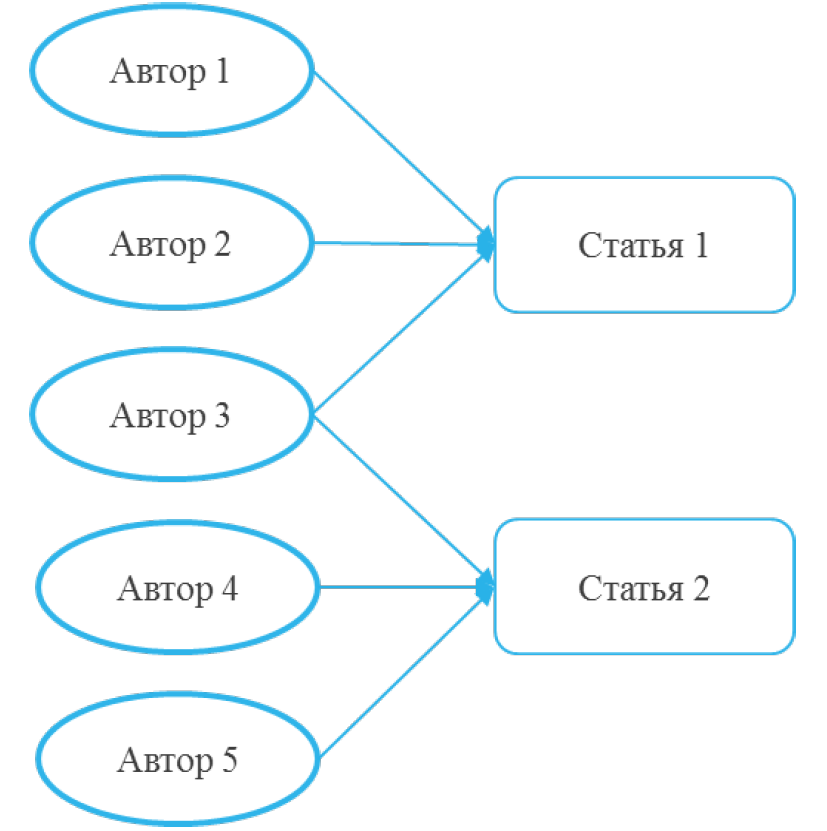
\includegraphics[width=0.8\textwidth]{bi_fig1}
  \label{fig:bi1}
  \caption{Двудольный граф соавторств.}
\end{figure}  
 
Преимущества такого подхода состоят в том, что в графе соавторств становится возможным сохранить для дальнейшего анализа библиографическую информацию о статье: 

\begin{enumerate}
\tightlist
\item Название статьи 
\item Год издания 
\item Издатель 
\item Ключевые слова 
\end{enumerate}

Отметим, что традиционное представление графа соавторств в виде неориентированного графа является проекцией двудольного графа на множество вершин авторов. 
Поясним это более подробно. 
Ориентированный граф $G = (V,E)$  называется двудольным, если множество его вершин можно разбить на две части $ A \cup P = V$, так, что 
\begin{itemize}
	\item ни одна вершина в $A$ не соединена с вершинами в $P$
	\item ни одна вершина в $P$ не соединена с вершинами в $A$. 	
\end{itemize}

В рассматриваемом случае $A$ - это множество авторов, $P$ - это множество статей. $A$ и $P$ - являются долями графа $G$.
Отметим, что граф $G$ может быть как полным так и неполным в зависимости от того имеют ли авторы соединения со всеми статьями. 
Приведенный на Рисунке \ref{bi_fig1} двудольный граф является неполным. 
Обозначим  $G_A$ проекцию графа  $G$ на множество вершин $A$.
Граф $G_A$ является традиционным представлением графа соавторств и отображен на рисунке \ref{fig:bi2}. 

\begin{figure}[H]
  \centering
    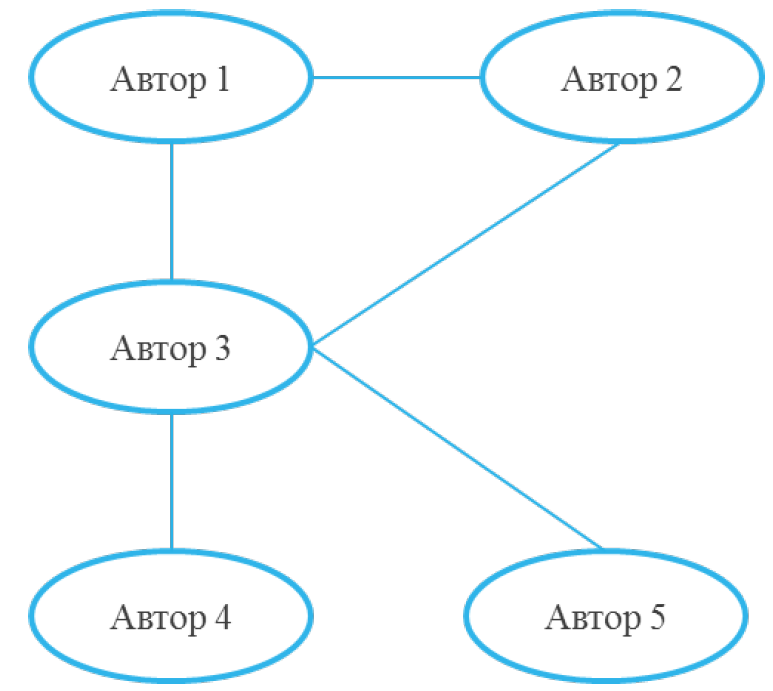
\includegraphics[width=0.8\textwidth]{bi_fig2}
  \label{fig:bi2}
  \caption{Неориентированный граф соавторств.}
\end{figure}  

Из рисунка \ref{fig:bi2} видно, что при построении проекции атрибутами ребер графа $G_A$ могут стать только интегральные характеристики соавторства, например, количество соавторств двух авторов.

\subsection{Моделирование графов соавторства}
Для моделирования графов соавторства как социальной сети широко применяется следующие стохастические подходы: 
\begin{enumerate}
\item Случайные графы.
\item Модель ``Маленький мир'' (small-world).
\item Модели, основанные на концепции преимущественного присоединения (preferential attachment).
\end{enumerate}

Одним из существенных ограничений стохастических моделей является фиксированное количество рассматриваемых вершин, или их постоянный рост. 
На практике в организации изменяется количество потенциальных соавторов.
Так же важно понимать, что стохастические модели ставят целью моделировать граф с определенными параметрами. 
Такими как, кластеризация, плотность и др.

С другой стороны, формирование малых групп, к которым относится и группа соавторов научной статьи, моделируется на основании принципа дополнительных компетенций, относящегося к классу детерминированных методов создания графов соавторства. 

Для предсказания новых вершин графа соавторства применяется комбинированный подход на основе машинного обучения с предварительным отбором признаков авторов, статистических показателей активности за несколько последних временных промежутков, а также структурные индексы влияния и локальные метрики в сети соавторства. 
Полученные в данной работе результаты позволили сделать вывод о применимости методов предсказания связей для анализа коллаборативных шаблонов поведения в крупной организации с динамической структурой коллектива, а также меняющимися внешними и внутренними факторами, влияющими на индивидуальную и коллективную публикационную активность.

Основой для прогнозирования изменений графа соавторств для научно-технического центра являются следующие компоненты: 
\begin{itemize}
\item Текущая структура графа соавторств.
\item Внешние по отношению к научно-техническому центру воздействия.
\item Внутренние изменения научно-технического центра. 
\end{itemize}

Рассмотрим каждую из компонент подробнее. Текущая структура графа соавторств представляет набор метрик, описывающих данный граф соавторств.
К таким метрикам принято относить следующие: 
\begin{itemize}
\item Для ребер
\begin{itemize}
\item Common Neighbours (CN)
\item Salton Index (SI)
\item Jaccard Index (JI)
\item Hub Promoted Index (HPI)
\item Hub Depressed Index (HDI)
\item Leicht-Holme-Newman Index (LHN1)
\item Preferential Attachment Index (PA)
\item Adamic-Adar Index (AA)
\item Resource Allocation Index (RA)
\end{itemize}
\item Для вершин 
\begin{itemize}
\item Degree centrality
\item Betweenness centrality
\item Closeness centrality
\item Harmonic centrality
\item Clustering
\end{itemize}
\end{itemize}

Каждая из этих метрик представляет характерный набор признаков (features) графа соавторств, влияющих на прогноз его изменений. 
Внешние по отношению к научно-техническому центру воздействия заключаются в публикационной политике редакций, публикующих научные статьи. 
В простейшем случае отсутствие возможности опубликовать статью из-за ограничений по объему выпуска журнала приводит несостоявшемуся соавторству. 
Основные зависимости публикационной активности научно-технического центра от редакций рассмотрены в работе \cite{krasnov2017model}.
Внутренние изменения научно-технического центра вызваны изменениями в составе персонала. 
В организацию приходят новые сотрудники, некоторые сотрудники увольняются.
В процессе наставничества и обучения сотрудники приобретают новые компетенции. 
В результате проведения НИР рождаются новые исследования и научные заделы. 
Часто, изменения внутренних требований к качеству публикаций также могут стать причиной структурных изменений, подтверждая принцип “publish or perish”, и влияя как на структуру коллектива, так и на параметры активности отдельных сотрудников и исследовательских коллективов.
Рассмотрим подробнее в чем состоит прогноз развития графа соавторств для научно-технического центра. 
Под развитием будем понимать возникновение новых вершин и ребер. 
Граф соавторств может рассматриваться как накопленным итогом за период, так и инкрементальными изменениями по годам. 
Далее будем рассматривать факт авторства, как признак вершины графа соавторств.
Другими словами, сотрудник, представляемый вершиной графа соавторства, может как написать, так и не написать статью в следующем временном периоде. 
Процесс прогнозирования в данном случае будет решать задачу бинарной классификации. 
Для каждого сотрудника будет определяться вероятность создания статьи по определенной тематике. 
Статья является коллективным усилием работы соавторов, обладающих определенным набором компетенций, нашедших свое применение в цели исследования.
В этом состоит основная идея принципа дополнительности компетенций. 
Авторы с одинаковыми компетенциями не имеют рационального обоснования для объединения с целью проведения научного исследования. 
Будем считать, компетенции атрибутами вершин графа.  
Для выявления компетенций необходимых для написания статьи будем использовать ключевые слова, а при их отсутствии – метод тематического моделирования текста работы.

\section{Современные процессы организации труда на основе гибких методик}

Гибкие (Agile) методики разработки программного обеспечения широко применяются в различных индустриях. 
Написание программного кода по своей сути является процессом создания логически структурированного текста так же, как и написание научной статьи. 
Коллективная работа над написанием научных статей требует разделения обязанностей для повышения продуктивности так же, как и написание программного кода требует выделения специалистов для тестирования и документирования.

Использование ролевой модели гибких методик представляется перспективным кросс-индустриальным опытом для применения, но нуждается в теоретической проверке. Одним из вариантов проверки гипотез, показавшим себя в условиях, когда постановка реального эксперимента представляется высоко затратной, является метод имитационного моделирования. 
Автор видит дополнительные преимущества от институциализации процесса написания научных статей и применения проверенных индустриальных показателей эффективности для его оценки.

Провозглашение основных принципов гибких методик в виде манифеста \cite{fowler2001agile} обозначило насущную необходимость перехода к более эффективным методам разработки программного обеспечения. 
Решительность этого шага многократно себя оправдала на практике и в последствии нашла теоретические обоснования {bonner2016empirical}. 
Суть гибких методик может быть изложена по-разному, но для данного исследования нами выбрана следующая формулировка:

\begin{enumerate}
\tightlist
\item Приоритет командных взаимодействий
\item Приоритет работающего программного кода
\item Приоритет реакций над планом
\end{enumerate}

Современные методики написания научных статей остаются на позициях последовательного, ``водопадного'' подхода.
Такой подход был уместен во времена Ньютона, когда один уникальный ум работал над трудом всей своей жизни.
В условиях современной скорости обмена научной информацией одиночки остаются не у дел.
Им на смену приходят научные коллективы.
Интуитивно понятно, что от согласованной работы научного коллектива соавторов зависит их продуктивность: оптимальное соотношения качества и скорости публикации результатов научных исследований в виде научных статей, доступных наиболее широкому кругу заинтересованных лиц. 
В гибких методиках разработки программного обеспечения образование команды основано на принципах самоорганизации \cite{hoda2016multi,moe2008understanding}.
Самоорганизующиеся команды  в работе \cite{moe2009overcoming} разделены на три типа:

\begin{enumerate}
\tightlist
\item  ``Команда пилотов самолёта'': Управление воздушным судном.
\item  ``Компьютерные команды'': Создание новых программных продуктов.
\item  ``Команда КВН'': Решение сложных проблем.
\end{enumerate}

Для целей дальнейшего исследования нас больше будут интересовать тип ``Компьютерные команды''.

\subsection{Размеры команд}

Размеры команд играют важную роль. 
В гибких методиках разработки программного обеспечения рассматриваются малые (5-7), большие (10-50) и сверхбольшие команды (100-200) \cite{alnuaimi2010team}.

Важно отметить, что приведенные оценки сходятся с полученными в работе \cite{kradoya2016structure} для команд соавторов: современные творческие команды соавторов в среднем состоят из 3 участников. 
В дальнейшем изложении будем подразумевать, что число участников команды состоит в среднем из 3 соавторов.

\subsection{Образование команд}

Гибкие методики \cite{fowler2001agile} подразумевают под самоорганизацией только возможность работы команды с ограниченным управлением из вне. 
На взгляд автора данного исследования, целесообразно рассмотреть, как образуются команды в деталях.

Для рассмотрения механизма необходимо понимать, что команда образуется с определённой целью. 
Рассматривая образование команд авторы исследования \cite{guimera2005team} предлагают эмпирический вероятностный алгоритм присоединения нового участника к уже сформированной группе (Рис.\ref{ex:fig2_1}):

\begin{figure}[H]
  \centering
    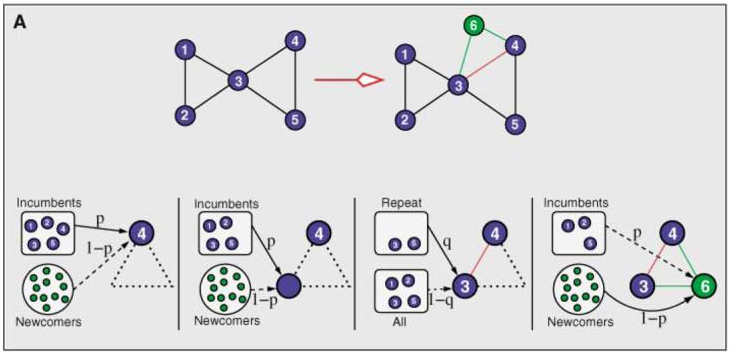
\includegraphics[width=0.8\textwidth]{guimera2}
  \label{ex:fig2_1}
  \caption{Алгоритм образования команд на основе вероятностей (p - для новых участников, q - для участников группы) \cite{guimera2005team}}
\end{figure}
 
Таким образом, авторы работы \cite{guimera2005team} оценивают влияние внутренней структуры команды на её расширение.

В работе \cite{moe2009overcoming} отмечено, что основным фактором для самоорганизации команд являются индивидуальные компетенции.
При этом компетенции каждого участника оцениваются с точки зрения полезности для достижения цели. 
В исследованиях \cite{berger1972status,berger1980status} утверждается, что такая оценка приводит к появлению системы статусов участников команды, которая выражается в иерархичности коммуникаций. 
Для настоящего исследования нам достаточно того, что:
\begin{enumerate}
\tightlist
\item  Цель является образующим базисом для команды;
\item  Цель декларирует потребности в компетенциях участников команды;
\item  Участники производят оценку компетенций друг друга для достижения цели.
\end{enumerate}

Базовый алгоритм образования команды для двух участников может быть представлен в виде следующей временной последовательности (\ref{ex:fig2}):

\begin{figure}[H]
  \centering
    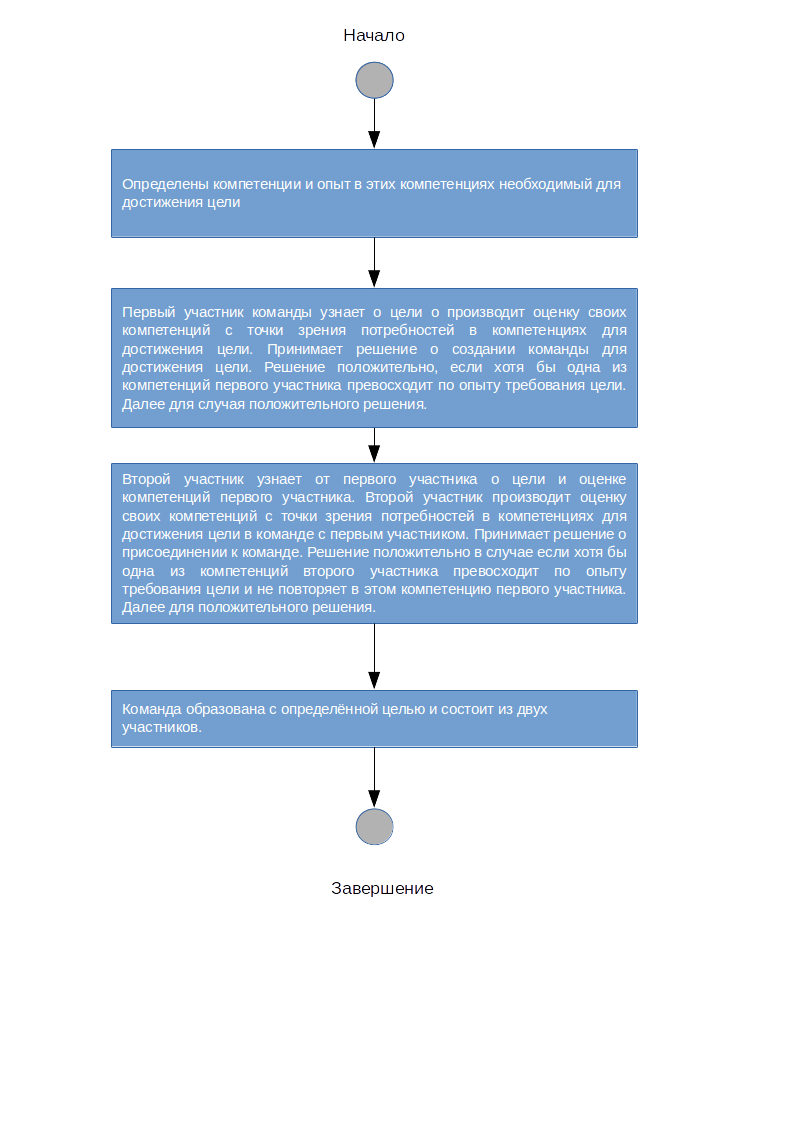
\includegraphics[width=0.8\textwidth]{ex_fig2}
  \label{ex:fig2}
  \caption{Базовый алгоритм образования команды.}
\end{figure}


Приведенная на Рис. \ref{ex:fig2} последовательность описывает основное образующее команду действие - \textit{парное объединение}.
Можно сказать, что после присоединения участников у команды появляется собственный профиль компетенций для достижения заданной цели. 
Компетенции команды получаются в результате суперпозиции компетенций участников. 
Некоторые из компетенций необходимых для достижения цели ``закрыты опытом'' участников, а некоторые нет.
Следующий за первым участник присоединяется уже с учётом профиля компетенций команды. 
Для удобства дальнейшего изложения сформулируем следующие утверждения:

\begin{state}[У\ref{state:1}] \label{state:1}
Сотрудники объединяются в команду для достижения цели.
\end{state}

\begin{state}[У\ref{state:2}] \label{state:2}
Компетенции команды являются функцией от компетенций участников.
\end{state}

\begin{state}[У\ref{state:3}] \label{state:3} 
Объединение первого участника с командой
для достижения цели происходит по таким же принципам, что и объединение
команды из n участником с n+1 участником. 
\end{state}

\subsection{Парное объединение}

Рассмотрим подробнее \emph{парное объединение}. 
Организационная среда задает размерность $N_{comp}$ пространства компетенций. 
Каждый участник организационной среды $a$ обладает вектором компетенций $c_i$ таких, что $i \in N_{comp}$. 
Каждая компетенция участника $c_i$ характеризуется опытом $e_i$ . 
Опыт участника -- это натуральное число, $e_i \in \mathbb{N}$. 
В результате можно сказать, что  участник обладает вектором опыта в пространстве компетенций. 
Отметим, что пространство компетенций организационной среды обладает существенно большей размерностью, чем вектор компетенций участника.
Изначально команда $t_0$ не содержит участников и не обладает собственными компетенциями (Рис. \ref{ex:fig3}).

\begin{figure}[H]
  \centering
    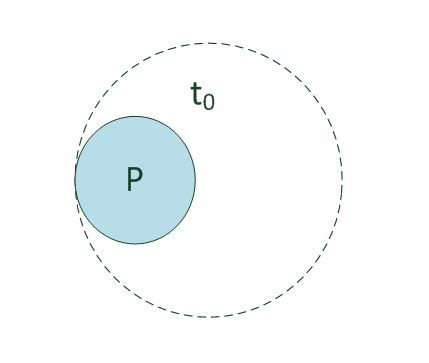
\includegraphics[width=0.5\textwidth]{scrum_fig3}
  \label{ex:fig3}
  \caption{Схема команды без участников.}
\end{figure}

Пусть $P$ обозначает цель для объединения команды, $c_j$ -- вектор компетенций, а $e_j$ -- опыт по каждой компетенции необходимый для достижения $P$. 
В результате успешного объединения для достижения цели будет образована команда $t_1$(Рис. \ref{ex:fig4}).

\begin{figure}[H]
  \centering
    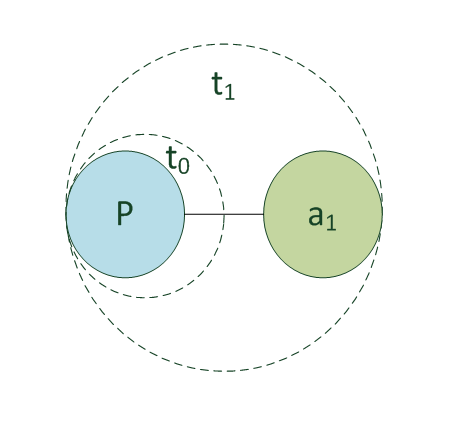
\includegraphics[width=0.5\textwidth]{scrum_fig4}
  \label{ex:fig4}
  \caption{Схема команды из одного участника.}
\end{figure} 

Команда $t_1$ обладает новым вектором компетенций. 
Так как в $t_1$ только один участник $a_1$, то вектор компетенций $t_1$ будет совпадать с вектором компетенций $a_1$. 
При присоединении к  $t_1$ участника $a_2$ будет образована команда $t_2$ (Рис. \ref{ex:fig5}).

\begin{figure}[H]
  \centering
    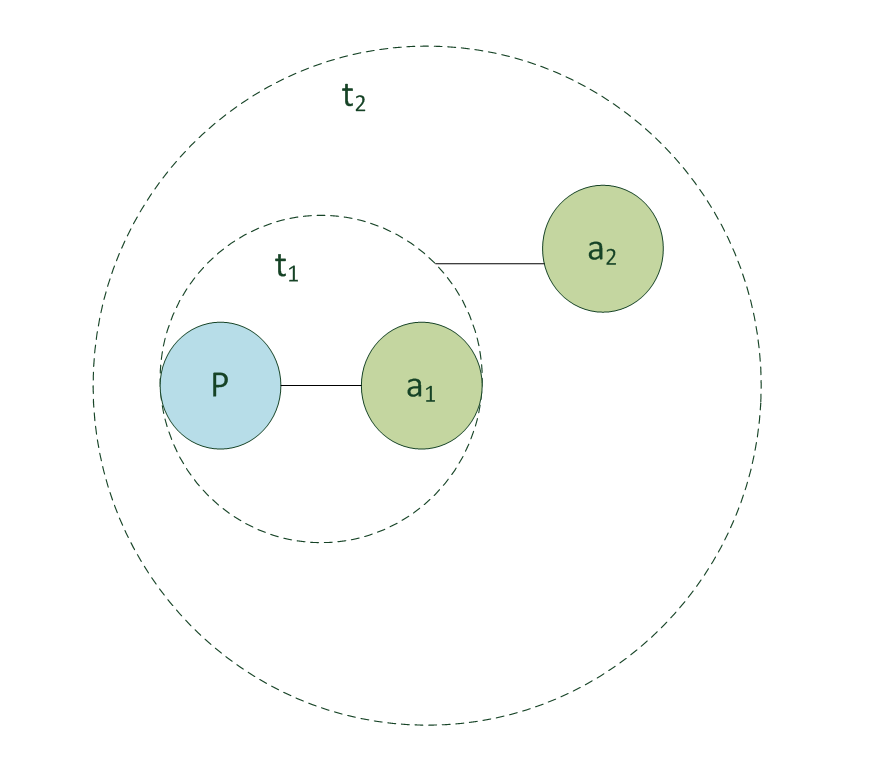
\includegraphics[width=0.8\textwidth]{scrum_fig5}
  \label{ex:fig5}
  \caption{Схема команды из двух участников.}
\end{figure} 


Так как участник присоединяется ко всем элементам команды , то можно привести схему (Рис. \ref{ex:fig5}) к виду графа команды (Рис. \ref{ex:fig6}).

\begin{figure}[H]
  \centering
    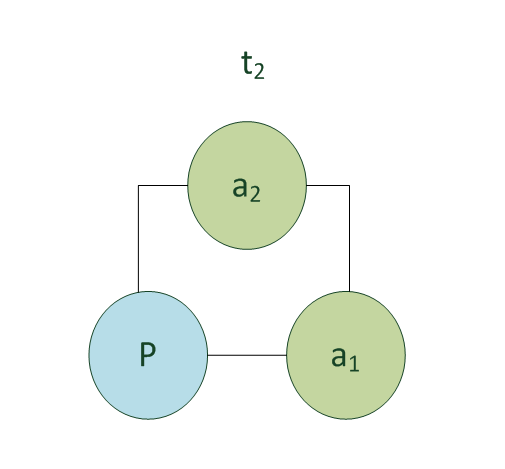
\includegraphics[width=0.8\textwidth]{scrum_fig6}
  \label{ex:fig6}
  \caption{Граф команды из двух участников с избыточными связями.}
\end{figure}  

Цель является $P$ атрибутом ребра, связывающего $a_1$ и $a_2$, поэтому можем преобразовать граф команды с двумя участниками к виду (Рис. \ref{ex:fig7}).

\begin{figure}[H]
  \centering
    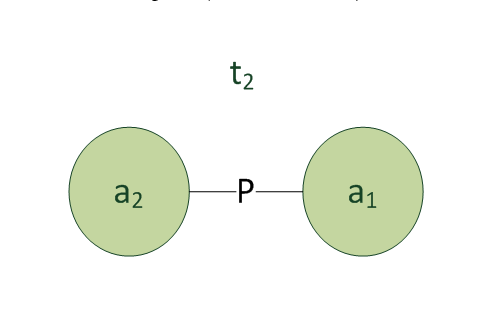
\includegraphics[width=0.8\textwidth]{scrum_fig7}
  \label{ex:fig7}
  \caption{Граф команды из двух участников.}
\end{figure}  

Для случая написания научных статей граф команды $t_2$, изображенный на Рис.\ref{ex:fig7} обозначают $g(t_2)$ и называют графом соавторства, где под $P$ подразумевают научную статью.
Информация о истории создания команды в такой нотации не приводится. 
На Рис.\ref{ex:fig8} приведен пример фрагмента графа соавторства.
Вершинами графа являются исследователями, а ребрами -- совместная научная публикация. 
Граф соавторства является ненаправленной сетью.
\begin{figure}[H]
  \centering
    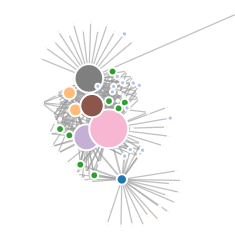
\includegraphics[width=0.5\textwidth]{scrum-img8}
  \label{ex:fig8}
  \caption{Фрагмента графа соавторства для нескольких команд.}
\end{figure}  

Отметим, что для наглядности на Рис.\ref{ex:fig8} размер вершин отражает количество научных статей, написанных участником.

\subsubsection{Командный код}

Введем понятия \emph{полного командного кода} \emph{(ПКК)} и \emph{остаточного командного кода (ОКК)}.
Эти понятия играют ключевую роль в образовании команды. 
Составляющими командного кода являются компетенции. По своему типу \emph{полный} и \emph{остаточный} \emph{командный код} -- это вектора в пространстве $N_{comp}$ .

Рассмотрим, как участником производится оценка своих компетенций с точки зрения потребностей в компетенциях для достижения цели.

Характеристики цели $P$ являются основанием для образования команды. 
То есть, первый участник команды $a$ и цель $P$ должны быть объединены на основании представления о компетенциях. 
Другими словами, необходимыми условиями для достижения цели должно быть обладание $a$ определенным набором компетенций и опыта. 
С точки зрения множеств компетенции сотрудника $a$ и цели $P$ должны находиться в одном пространстве и иметь пересечения. 
Наличие пересечений будет приводить к объединению в команду.

Введем функцию оценки в виде $\Phi(P,t,a), \Phi \in [0,1] $. 
Результатом $\Phi$ будет вероятность возможности объединения участника $a$  в команду $t$ для достижений цели $P$. 
Тогда функция $\Phi$ для $n$-ого участника может быть записана в виде $\Phi_n(P,t_{n},a_n)$.

По мере присоединения участника вектор компетенций команды будет изменяться.
В него будут входить компетенции новых участников, а опыт по одинаковым компетенциям будет складываться.

\begin{equation} 
\label{eq:scrum1}
ut_{n-1} = \prod_{a_j}^{a_{n-1}}\sum_i^{N_{comp}}\bigg\{c_j * \, e_i \bigg\}
\end{equation}

Величину $ut_{n-1}$ будем называть \emph{полным командным кодом (ПКК)}. 
\emph{ПКК} характеризует потенциал команды для достижения целей.

В соответствии с вышеописанным алгоритмом (Рис. \ref{ex:fig2}) функцию $\Phi$ можно представить в виде:

\begin{equation} 
\label{eq:scrum2}
\Phi  = P \cdot \prod_{a_j}^{a_{n-1}}\sum_i^{N_{comp}} \bigg\{c_j *\, e_i \bigg\} \cdot a_n
\end{equation}

Важную смысловую часть в выражении (\ref{eq:scrum2}) несет компонент $rt^P_n$, который автор называет \emph{остаточным командным кодом}  -- \emph{ОКК}.

\begin{equation} 
\label{eq:scrum3}
rt_n^P  = P \cdot \prod_{a_j}^{a_{n-1}}\sum_i^{N_{comp}} \bigg\{c_j *\, e_i \bigg\}
\end{equation}

\emph{ОКК} $rt_n^P$ характеризует незакрытые $t_n$ командой компетенции цели $P$. 
Нулевой вектор в качестве \emph{ОКК} характеризует полную укомплектованность компетенциями команды для достижения цели.

С учетом \emph{ОКК} можно преобразовать выражение (\ref{eq:scrum2}) следующим образом:

\begin{equation} 
\label{eq:scrum4}
\Phi  =  rt_n^P \cdot a_n 
\end{equation}

Выражение (\ref{eq:scrum4}) имеет интуитивно понятный смысл: 
\emph{для оценки возможности присоединения к команде новый участник должен выяснить обладает ли он необходимым опытом в требуемых для выполнения цели компетенциях с учетом того, что существующая команда уже закрыла часть из необходимых компетенций своим опытом}. 
В работах \cite{hamilton2003team,prat2002should} такой принцип образования команд называют комплементарным.

\subsubsection{Гомогенность команд}

Мы рассмотрели образование команд на основе дополнительности (комплементарности) компетенций. 
Второй движущей силой для образования команд является гомогенность.

Гомогенность групп в социальных сетях, или склонность людей со схожими характеристиками формировать связи между собой, также называемая гомофилией, является важным фактором формирования и эволюции социальных сетей \cite{mcpherson2001birds}. 
Во многих работах отмечается динамическая структура гомофилии \cite{snijders2010introduction,steglich20108}, в ходе которой параллельно происходят два процесса.
С одной стороны -- схожие между собой индивиды формируют социальные связи (социальная селекция). 
С другой -- уже связанные друг с другом люди перенимают поведение друг друга (социальное влияние).
Совокупность этих факторов результирует в гомогенную социальную систему, в которой между индивидами со схожим поведением и характеристиками есть связь, при этом характер связи может быть, как формальным, так и неформальным.

Несмотря на то, что связи между индивидами со схожими характеристиками более вероятны, чем связи между непохожими, уровень схожести также важен.
В работе \cite{block2014multidimensional} было показано, что социальная схожесть более, чем по одному показателю, приводит к тому, что люди с меньшей вероятностью будут формировать между собой взаимоотношения. 
Автор объясняет данный эффект тем, что слишком схожие по многим характеристикам люди, как правило, не могут привести что-то новое и конструктивное во взаимные отношения или же в команду.
Для продуктивного сотрудничества необходима не только схожесть интересов, но также и различный профессиональный и жизненный опыт, позволяющий предложить многомерные подходы к ее решению.

Основным объединяющим фактором в команде являются компетенции участников, влияющие на достижения цели.
Основываясь на понятии \emph{ОКК}, введенного ранее, можно рассмотреть остаточные компетенции участника, то есть компетенции, не востребованные для объединения команду для достижения цели. 
Влияние этой части компетенций на команду может как усиливать ее, так и ослаблять во время работы.

\subsubsection{Работа команд}

Начало работ по достижению цели определяется участниками команды и не зависит от процесса образования команды. 
Показатели производительности могут быть только у работающей команды. 
Например, важное для научной сферы деятельности понятие \emph{научный} \emph{задел} означает ни что иное как работы, выполненные командой имеющей не пустой \emph{остаточный} \emph{командный код.}

Формирование основной системы внутреннего взаимодействия внутри команды согласно исследованию \cite{harper1985power} происходит при знакомстве участников.
Таким образом, для данного исследования будем пренебрегать временем установления устойчивой работы каналов коммуникаций.

В гибких методиках разработки программного обеспечения наибольшее внимание уделяется именно коммуникациям внутри команды \cite{boehm2003people} и с внешними агентами \cite{paasivaara2012experiences}, которые по сути тоже являются командой, но в более широком смысле.

Сформулируем следующее утверждение:

\begin{state}[У\ref{state:4}] \label{state:4}
Характеристики работы каналов коммуникаций соответствуют характеру работы команды.
\end{state}

Таким образом, измеряя работу коммуникационных каналов можно сделать заключения о характере работы команды.
Отметим, важное следствие: такой тип измерения производительности команды не создаёт дополнительной нагрузки на сотрудников в отличии от методик оценки основанных опросах.

Вопрос измерения вклада отдельных участников или результата команды рассмотрен в ряде работ \cite{tannenbaum2013team,hill1982group} и все исследователи склоняются к тому, что измерять нужно и командную производительность (Team Performance), и индивидуальная продуктивность (Individual Performance).
В исследовании \cite{tims2013job} приведена следующая схема измерений (Рис. \ref{ex:fig9}).

\begin{figure}[H]
  \centering
    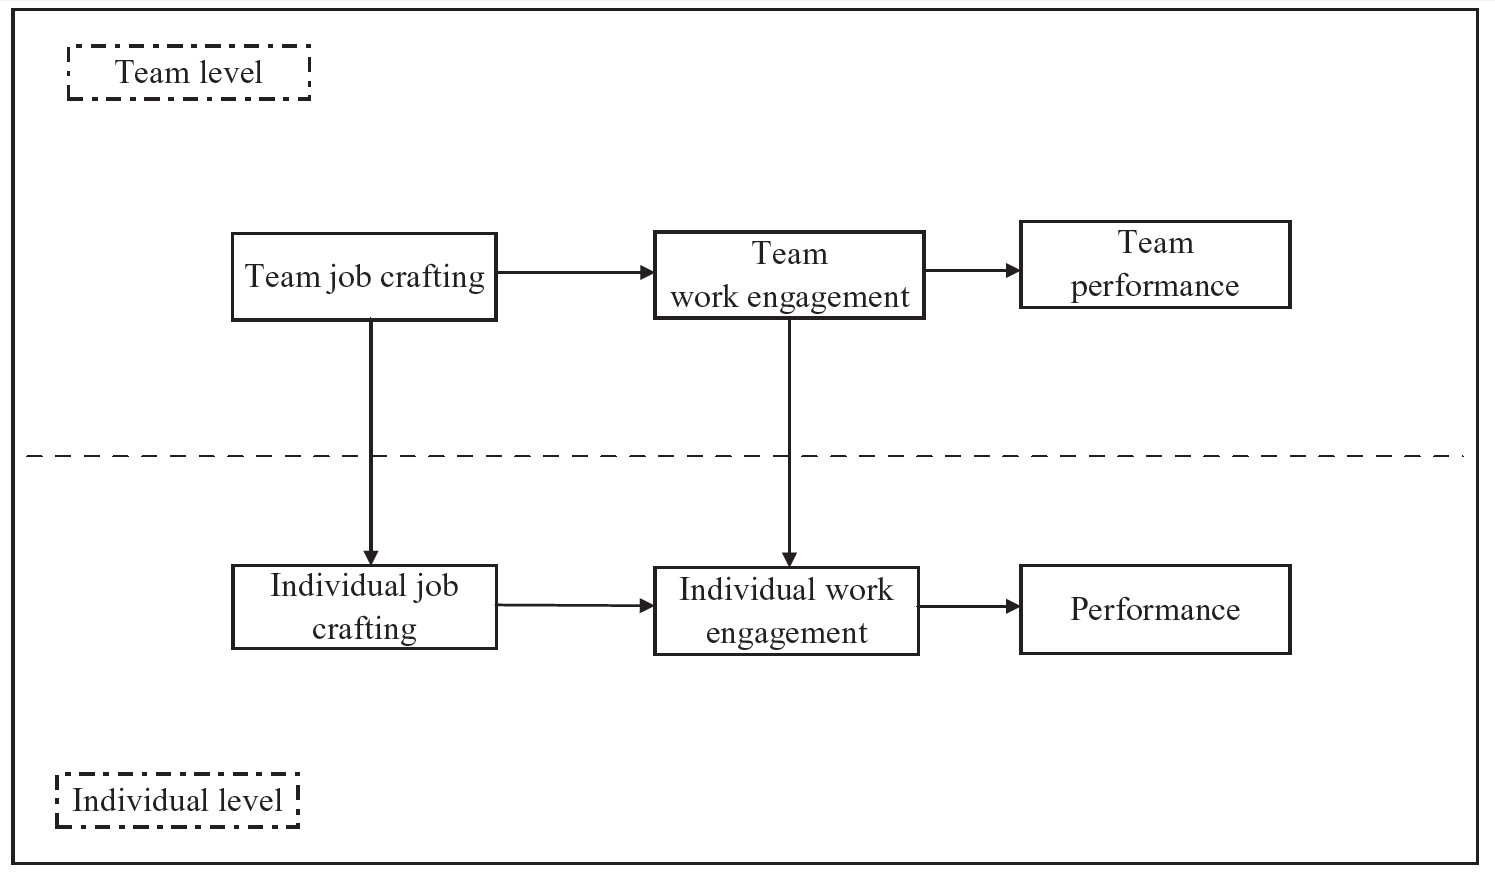
\includegraphics[width=0.8\textwidth]{scrum-img9}
  \label{ex:fig9}
  \caption{Уровни измерения производительности команды и участника \cite{tims2013job}.}
\end{figure}  

Например, измерение Individual Performance с помощью опросов исследуется в работе \cite{cropley2012measuring} путём введения Creative Solution Diagnosis Scale (CSDS) -- шкалы креативности. 
Измерить Individual Performance сотрудника по такой шкале авторы \cite{cropley2012measuring} предлагают с помощью Consensual Assessment Technique (CAT), которая требует дополнительных усилий от сотрудников.
Сильные и слабые стороны метода опросов для измерения Individual Performance изложены в фундаментальной работе \cite{jackson1965person}.

Вопрос метода измерения Individual Performance находит интересную постановку в современной концепции ``sensible organization'' \cite{olguin2008sensible}.
Авторы исследования \cite{olguin2008sensible} помимо измерения традиционных цифровых коммуникационных каналов надевают на сотрудников браслеты, отслеживающие перемещения и другие параметры организма.

Вопросы зависимости производительности команд от структуры команд рассмотрены в исследовании \cite{kradoya2016structure}.

\subsubsection{Методика Scrum}
Одной из распространённых гибких методик командной работы является методика Scrum \cite{sutherland2013scrum}. 
Scrum предназначен для получения наилучших из возможных результатов для командной разработки сложных интеллектуальных продуктов.
В классическом Scrum существует 3 базовых роли:

\begin{itemize}
\tightlist
\item  Product owner -- отвечает за соответствия целям
\item  Scrum master -- отвечает за эффективное взаимодействие в команде
\item  Команда разработки (Development team)
\end{itemize}

Рекомендуемый размер Scrum команды --- 5-7 человек соответствует принятым в данном исследовании ограничениям.
Согласно идеологам Scrum \cite{sutherland2013scrum}, команды большего размера требуют значительных ресурсов на коммуникации, в то время как команды меньшего размера уменьшают размер работы, который команда может выполнить в единицу времени.

Основой Scrum является Sprint, в течении которого выполняется работа над продуктом. 
Sprint имеет одинаковую продолжительность на протяжении всего процессы создания продукта, рекомендуется одна неделя. 
Задача Sprint состоит в том, чтобы материализовать продукт в текущем виде. 
Продуктом в данном исследовании является научная статья.

Методика Scrum декларирует необходимость в определенных видах деятельности, не связанных с исследованиями и написанием текста, которые приводят к лучшей результативности. 
Кроме этого Scrum задает определенный ритм для этих дополнительных деятельностей.

Введем показатели, на которые влияет применение Scrum к процессу написания научных статей:

\begin{enumerate}
\tightlist
  \item   Ускорения обмена сообщениями в каналах коммуникаций;
  \item   Потеря работ из-за дублирования при отсутствии своевременных коммуникаций о прогрессе проведения исследований;
  \item   Потеря работ из-за несоответствия написанной статьи правилам  публикации.
\end{enumerate}

С точки зрения формализма графа соавторства применение Scrum приведет к выделению вершин графа, обеспечивающих функции \emph{Product owner (PO)} и \emph{Scrum master (SM)} (Рис.\ref{ex:fig10})

\begin{figure}[H]
  \centering
    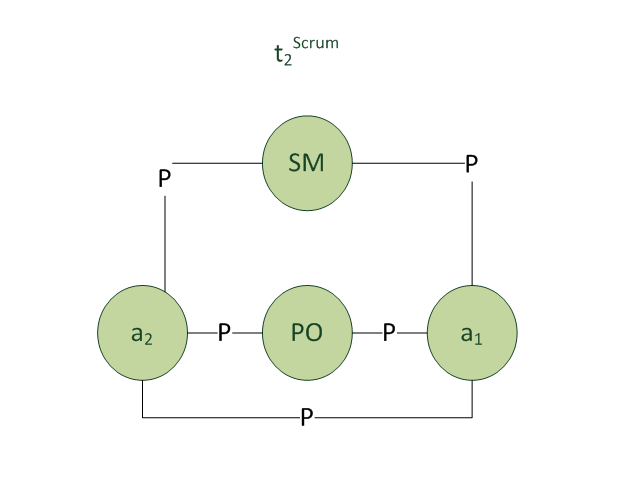
\includegraphics[width=0.8\textwidth]{scrum_fig10}
  \caption{Соавторство с ролями Scrum.}
  \label{ex:fig10}
\end{figure}  

С графом $g(t_2^{Scrum}$), отображенным на Рис.\ref{ex:fig10} можно произвести преобразование аналогичное сделанному выше с графом $g(t_2)$. 
Как мы видим, Scrum роли PO и SM соединяют вершины $a_1$и $a_2$. 
Из чего следует, что PO и SM являются характеристиками ребер графа, соединяющего $a_1$ и $a_2$. 
Преобразованный граф соавторства с применением Scrum ролей отображен на Рис. \ref{ex:fig11}.

\begin{figure}[H]
  \centering
    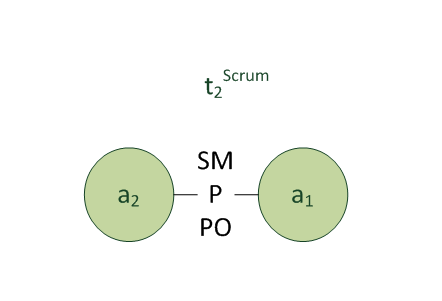
\includegraphics[width=0.8\textwidth]{scrum_fig11}
  \caption{ Граф соавторства с атрибутами Scrum.}
  \label{ex:fig11}
\end{figure}  

Роли Scrum согласно \cite{fowler2001agile} не должны вмешиваться в содержательную часть работы команды, а лишь ускорять информационный обмен и устранять информационные барьеры.
Сформулируем это в виде гипотезы, формальное доказательство которой отложим для дальнейших исследований:

\begin{hyp}[Г\ref{hyp:ex1}] \label{hyp:ex1}
Введение ролей Scrum в процесс соавторства не изменяет вид графа соавторства.
\end{hyp}

Теперь рассмотрим показатели производительности работы команд.

\subsubsection{Показатели производительности команд}

В современной работе \cite{pereme2016toward} рассмотрены вопросы разработки показателей, измеряющих скорость перехода продукта из фазы исследований (research) в фазу разработки (development). 
Авторами \cite{pereme2016toward} предложена интегральная модель для таких показателей. 
Объектом измерения авторы считают знания, а показатели основывают на процессе Knowledge Management. 
Никаких конкретных KPI авторы не предлагают, но описывают пространственные оси своей модели -- процессы, инструменты и люди.

Связь между способностью команды собраться и ее продуктивностью исследовали в работе \cite{edwards2006relationships}. 
Стоит отметить, что в работе \cite{edwards2006relationships} образование команды подразумевает формирование, а не самоорганизацию.

Состав команды во времени не постоянен и говорить от том, что образование команды в тот или иной момент времени завершено не корректно.
Участники могут покидать команду и участвовать в нескольких командах одновременно. 
Важная веха в работе команды определяется нулевым \emph{ОКК}, когда все компетенции необходимые для достижения цели представлены участниками команды. 
Сформулируем это в виде утверждения:

\begin{defi}[О\ref{defi:ex1}] \label{defi:ex1}
Команда считается укомплектованной, тогда и только тогда, когда ее ОКК равен нулевому вектору в пространстве $N_{comp}$.
Минимальное время, в котором ОКК стал равен нулевому вектору называется Временем комплектации ($T_c$).
\end{defi}

Отметим, что $T_c$ может быть больше времени, отведенного издательством или программным комитетом научной конференции на подготовку. 
Таким образом, статья не будет обладать требуемыми качествами в срок и не будет принята к публикации.

Показатели, наиболее точно отражающие динамику выполнения работы, будут основываться на изменении в динамике всех параметров команды. 
Введем функцию применения командой опыта в определенных целью компетенциях: $E(P,t)$.
Факторами, негативно влияющими на $E$ будут сложность коммуникаций внутри команды $\Xi(g)$ и необходимость заниматься деятельностью, не направленной на создания научных статей $\Gamma(t)$ .

И $\Xi(g)$, и $\Gamma(t)$ будут увеличивать время, требуемое на написание научной статьи.
Таким образом, команда может не достигнуть цели в определенные сроки.

Сформулируем две рассмотренные причины не достижения командой цели:

\begin{defi}[О\ref{defi:ex2}] \label{defi:ex2}
Несостоявшейся научной статьей (ННС) будем считать статью, не уложившуюся во временные рамки публикационного процесса с требуемым качеством. 
\end{defi}

Отношение количества несостоявшихся статей ($Frac_{notpub}$) к количеству опубликованных статей является показателем производительности процесса написания научных статей.

Другим более очевидным показателем производительности является время, затраченное на публикацию научной статьи ($T_{pub}$).

\section{Анализ текста}
\label{sec:topicmodel}
\subsection{Анализ текста на основании тематик}
%% Topics
В последние годы бурно развиваются методики тематического моделирования. Недавние исследования привели к развитию нескольких основных направлений: вероятностного [1], на основе SVD [2] и генеративного [4].
Тематическое моделирование определяет каждую тему как распределение некоторого количества слов с определенными вероятностями. Большинство современных тематических моделей строятся на основе распределения Дирихле (LDA, Latent Dirichlet Allocation) [3].
Трудно представить, что настолько универсальное распределение как LDA будет одинаково хорошо работать для любых текстов. 
Необходимы тонкие настройки алгоритма на конкретный проблемный домен. 
Поэтому автор сосредоточился на основном мировом источнике для научно-практических статей нефтегазовой отрасли – библиотеке OnePetro. 
Важно отметить, что OnePetro охватывает широкий спектр инженерных дисциплин и содержит тексты на английском посвященные именно практическим аспектам применения новых технологий в нефтегазовой отрасли. 
Авторами этих статей являются сотрудники нефтяных компаний со всего мира.
%% 

Формальная постановка задачи тематического моделирования следующая. 
Пусть зафиксирован словарь терминов $W$, из элементов которого складываются документы, и дана коллекция $D$ документов $d \in D$. 
Для каждого документа $d$ известна его длина $n_d$ и количество $n_dw$ использований каждого термина $w$.
Пусть $\Phi=(\phi_{wt})$ - матрица распределений терминов ($w$) в темах ($t$), а  $\Theta=(\theta_{td})$  - матрица распределений тем ($t$) в документах ($d$). 
Тогда задача тематического моделирования состоит в том, чтобы найти такие матрицы  $\Phi$ и $\Theta$, чтобы выполнялось равенство (\ref{eq:op3_1}).

\begin{equation} 
\label{eq:op3_1}
p ( w \vert d ) = \sum_{t \in T} \phi_{wt} \theta_{td},
\end{equation}
где $ \phi_{wt} $ - вероятности терминов $w$ в каждой теме $t$, $\theta_{td}$ – вероятности тем $t$ в каждом документе $d$, а $ p ( w \vert d ) $ – вероятность появления термина $w$ в документе $d$.

Уравнение (\ref{eq:op3_1}) можно представить в матричном виде $ \Phi \cdot \Theta $. 
При этом легко показать, что данная задача имеет много решений (\ref{eq:op3_2}). 
\begin{equation} 
\label{eq:op3_2}
\Phi \cdot \Theta  = \Phi \cdot \Lambda \cdot \Lambda^{-1} \cdot \Theta = \hat{\Phi} \cdot \hat{\Theta},
\end{equation}
где $\hat{\Phi} = \Phi \cdot \Lambda $, а  $\hat{\Theta} = \Lambda^{-1} \cdot \Theta$.

Из уравнения (\ref{eq:op3_2})  следует, что матрицы $\hat{\Phi}$ и $\hat{\Theta}$ так же будут являться решениями уравнения (\ref{eq:op3_1}).
Но не все матрицы $\Phi$ и $\Theta$ будут содержать хорошо интерпретируемые тематики. 
Таким образом, в задачу (\ref{eq:op3_1}) необходимо ввести условия способствующие получению адекватных и интересных тематик. 
Образно можно сказать, что необходимо оцифровать специфику предметной области текста для встраивания в алгоритм поиска оптимальных матриц $\Phi$ и $\Theta$. 
Отметим, что при использовании LDA для создания тематической модели такой настройки на предметную область не производится.
Для решения подзадачи настройки тематической модели на предметную область автором использован механизм регуляризаторов. 

Пусть $p \left( t \right) $ — распределение тем в коллекции документов:
\begin{equation} 
\label{eq:op3_3}
p \left( t \right) = \sum_d p \left( d \right)  \theta_{td}
\end{equation}

Тогда полезным представляется регуляризатор на основе дивергенции Кульбака-Лейбнера: 
\begin{equation} 
\label{eq:op3_4}
\mathcal{KL}(\Theta)= -\tau \sum_{t \in T} \ln \bigg( \sum_{d \in D} p \left( d \right) \theta_{td} \bigg) \rightarrow max
\end{equation}

Где $\tau$ – параметр регуляризации, который нужно подобрать в зависимости от предметной области коллекции документов. 
Требование максимизации $\mathcal{KL}(\Theta)$ будет означать обнуление вероятностей появления документов и приведет к большей разрежённости матрицы $\Theta$.
Вторым механизмом для регуляризации может быть обратное действие – увеличение вероятностей для тематик, которые присутствуют во многих документах. 
Такие тематики называют шумовыми. 
Для получения уплотнений строк матрицы  $\Theta$  с шумовыми тематиками можно применить регуляризатор (\ref{eq:op3_4})  с обратным знаком. 
Таким образом, матрица $\Theta$ после регуляризации будет представлять чередование зон разрежённости для основных тематик и уплотнений для шумовых тематик. 

Полученную тематическую модель необходимо формально проверить на качество. 
Для этого в процесс обучения необходимо встроить метрики качества модели. 
А после достижения формальных критериев сходимости на основании метрик провести визуализацию модели для общего контроля качества. 
Основной метрикой для выявления факта сходимости модели тем является метрика Perplexity вычисляемая по формуле (\ref{eq:op3_5}).

\begin{equation} 
\label{eq:op3_5}
\mathcal{P}(D, \Phi, \Theta) = \exp \bigg( \frac{-1}{n_d} \sum_{d \in D}  \sum_{w \in d}  n_{dw} \ln \bigg( \sum_{t \in T} \phi_{wt} \theta_{td} \bigg ) \bigg)
\end{equation}

Метрика Perplexity не нормирована и поэтому не может быть использована для сравнения сходимости разных моделей. 
Общая логика состоит в том, что чем меньше Perplexity, тем лучше модель. 
Поэтому для принятия решения о достаточной сходимости модели руководствуются тем, что Perplexity перестает значительно уменьшаться с ростом количества итераций обучения.

Результирующая модель тематик может быть рассмотрена как мягкая кластеризация. 
В таком случае к полученным тематикам могут быть применены инструменты визуализации, используемые для кластеров. 
Например, могут быть применены методы обучения на основе многообразий (Manifold Learning): t-distributed Stochastic Neighbor Embedding (TSNE)  и Multidimensional scaling. 
Результаты работы алгоритма TSNE зависят от выбранной метрики расстояния между векторами. 
При размерности векторного пространства в несколько сотен применяют следующие метрики: 

\begin{itemize}
\item 	Косинусная мера (Сosine): $ \frac{v_1 \cdot v_2}{\Vert v_1 \Vert_2 * \Vert v_2 \Vert_2 } $
\item 	Евклидово расстояние (Euclidean):$ \Vert v_1 - v_2 \Vert_2$
\end{itemize}

Для эффективного использования визуализации тематической модели с помощью методов обучения на основе многообразий необходимо представить слова, составляющие тематики, в векторном пространстве (Vector Space Model). 
Такая процедура называется word embedding. 
Для нее часто используют метод GloVe описанный в исследовании \cite{pennington2014glove}. 
Альтернативным методом word embedding является FastText \cite{joulin2016bag}, поэтому автор данного исследования решил провести качественное сравнение обоих методов word embedding на выбранной коллекции. 
Оба метода обучают векторные представления слов на основании того, как часто слова употребляются вместе. 
Отличие между ними состоит в том, что FastText условно можно назвать ``предиктивной'', а GloVe основывается только на частотах слов. 
В этом свете GloVe гораздо проще, а автор данного исследования верит, что простота в бизнесе — это залог эффективности.

Библиотека BigARTM \cite{ianina2017multi} позволяет выстраивать последовательно несколько регуляризаторов и управлять группами тематик. 
Такой инструмент является уникальным на момент написания данного исследования. 
Широко используемые на западе методы построения topic models на основе LDA не дают таких возможностей.

\subsection{Анализ эмоциональной окраски текстов}
Анализ тональности текста предназначен для выявления в текстах эмоционально окрашенной лексики. 
Иногда исследователи выделяют термин Opinion mining, подчеркивая тем самым задачу поиска в текстах оценочных суждений. 
Кроме академического изучения тональности текста как одного из разделов компьютерной лингвистики существует ряд прикладных исследований, направленных на улучшение процесса принятия управленческих решений.

Применение рекуррентных и сверточных нейронных сетей для анализа тональностей позволило достичь значительно большей точности по сравнению с моделями основанными логистической регрессии.

Автор сфокусировался на методике выбора оптимальной архитектуры и гиперпараметров нейронной сети, позволяющие обучить классификационную модель на публичном наборе данных, содержащем оценочные суждения, и затем предсказать фрагменты текста из научно-практических статей, содержащие оценочные суждения с заданной степенью точности.

Примененные автором методические подходы могут быть представлены в следующем методическом каркасе исследования (Рис. \ref{fig:op4_1}). 
Рассмотрим более подробно каждый из элементов методического каркаса.

\begin{figure}[H]
  \centering
    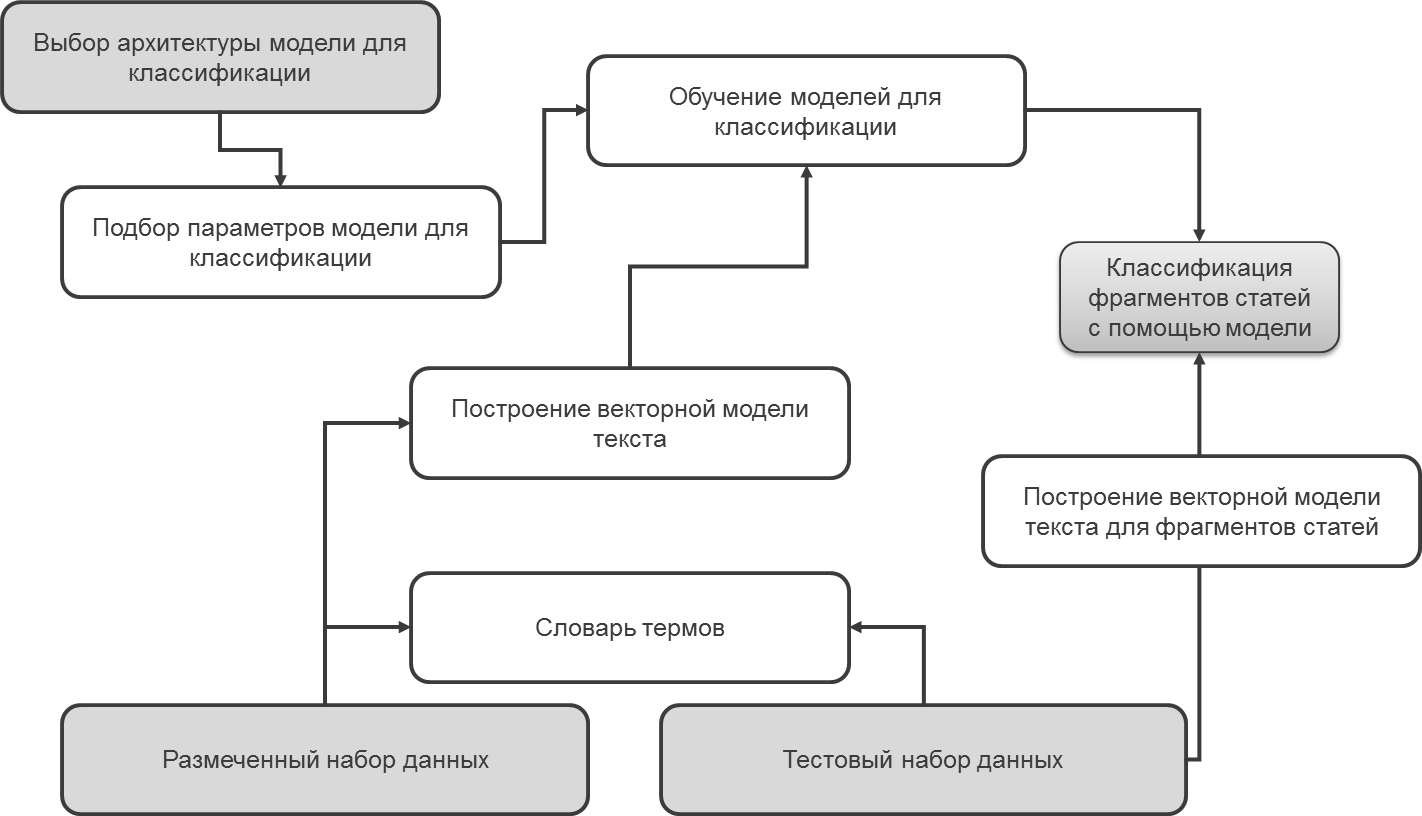
\includegraphics[width=0.8\textwidth]{op4_1}
  \label{fig:op4_1}
  \caption{ Методический каркас исследования эмоциональной окраски текстов.}
\end{figure}  
